\documentclass{article}
\pagenumbering{arabic}
\usepackage{graphicx,amsmath,amssymb,bm,tikz}
\usetikzlibrary{calc,patterns,decorations.pathmorphing,decorations.markings}
\usepackage{xfrac}
\usepackage[utf8]{inputenc}
\usepackage{hyperref}
% Format fref 
\usepackage[plain,english]{fancyref}
\usepackage[margin=1in]{geometry} 
\fancyrefaddcaptions{english}{\renewcommand*{\frefeqname}{Eq.}}
% Figure Packages
\usepackage[outercaption]{sidecap}
\usepackage[export]{adjustbox}
\usepackage{graphicx}
\usepackage{caption}
\usepackage{wrapfig}
\usepackage{float}
\usepackage{algorithm, algorithmic, amsfonts,amsmath,amssymb,amsthm, color,comment,enumitem, environ, fancyhdr,   graphicx, mathtools, wasysym}
\pagestyle{fancy}
\setlength{\headheight}{22.5pt}
\newenvironment{problem}[2][Problem]{\begin{trivlist}
\item[\hskip \labelsep {\bfseries #1}\hskip \labelsep {\bfseries #2.}]}{\end{trivlist}}
\newenvironment{sol}
    {\emph{Solution:}
    }
    {
    \qed
    }
\specialcomment{com}{ \color{blue} \textbf{Comment:} }{\color{black}} %for instructor comments while grading
\NewEnviron{probscore}{\marginpar{ \color{blue} \tiny Problem Score: \BODY \color{black} }}
%%%%%%%%%%%%%%%%%%%%%%%%%%%%%%%%%%%%%%%%%%%%%%%%%%%%%%%%%%%%%%%%%%%%%%%%%%%%%%%%%





%%%%%%%%%%%%%%%%%%%%%%%%%%%%%%%%%%%%%%%%%%%%%
%Fill in the appropriate information below
\lhead{Daniel Agramonte}  %replace with your name
\rhead{MCHE 6390 \\ Project 1 - Prelab} %replace XYZ with the homework course number, semester (e.g. ``Spring 2019"), and assignment number.
%%%%%%%%%%%%%%%%%%%%%%%%%%%%%%%%%%%%%%%%%%%%%



% Table stuff
\usepackage{multirow}
%\usepackage{floatrow}
%	\floatsetup[table]{capposition=top}%puts table caption above
% Change \subsection title characteristics
    \usepackage[parfill]{parskip}   % forces parskip to not affect headings
    \usepackage{enumitem}           % used for editing itemize environment
    \usepackage{titlesec}
        \titleformat*{\section}{\Large\bfseries\titlerule\vspace{0.5em}}
% Quote blocks
    \usepackage{csquotes} % use environment 'displayquote'
% Misc document settings
    \title{\Huge MCHE 6390 Project 1 - Prelab Work} \author{Daniel Agramonte} \date{10.30.20}
    \setlength{\parindent}{0pt}
    \setlength{\parskip}{1em}
    \setlist{nosep, itemsep=0pt, parsep=0pt}
% Misc vocab commands
    \newcommand{\msalg}{{\fontfamily{cmtt}\selectfont ms83}}
    \newcommand{\lsq}{\emph{lsqnonlin}}
    \newcommand{\msalge}{{\fontfamily{cmtt}\selectfont MCHE\_6500\_NIST\_POLY}}
%
% MATLAB packages
%
\usepackage[framed,numbered]{matlab-prettifier}
\usepackage{textcomp}
\usepackage{listings}
%
% Matrix Spacing
%
\makeatletter
\renewcommand*\env@matrix[1][\arraystretch]{%
  \edef\arraystretch{#1}%
  \hskip -\arraycolsep
  \let\@ifnextchar\new@ifnextchar
  \array{*\c@MaxMatrixCols c}}
\makeatother
%
\begin{document}
\maketitle
\section*{Modeling}
\subsection*{Part 1}
We first present our first order, two dimensional model of the following system. We assume that each floor will only move laterally in plane, and that each floor is connected with bars in perfect fixed-fixed boundary conditions.
\\ \\
\begin{tikzpicture}
\tikzstyle{spring}=[thick,decorate,decoration={zigzag,pre length=0.3cm,post length=0.3cm,segment length=6}]
\tikzstyle{damper}=[thick,decoration={markings,  
  mark connection node=dmp,
  mark=at position 0.5 with 
  {
    \node (dmp) [thick,inner sep=0pt,transform shape,rotate=-90,minimum width=15pt,minimum height=3pt,draw=none] {};
    \draw [thick] ($(dmp.north east)+(2pt,0)$) -- (dmp.south east) -- (dmp.south west) -- ($(dmp.north west)+(2pt,0)$);
    \draw [thick] ($(dmp.north)+(0,-5pt)$) -- ($(dmp.north)+(0,5pt)$);
  }
}, decorate]
\tikzstyle{ground}=[fill,pattern=north east lines,draw=none,minimum width=0.75cm,minimum height=0.3cm]
% Mass 1
\begin{scope}[xshift=7cm]
\node (M) [minimum width=2.5cm, minimum height=2.5cm]{};
\draw (-3,1.25) rectangle (3,1.75);
\node [] at (0,1.5) {$m_1$};
\node (ground) [ground,anchor=north,minimum width=9.cm] at (M.south) {};
\draw ($(ground.north east)$) -- ($(ground.north west)$);
% Coordinate System
\draw [thick,gray,->] (3,1.5) -- (3.5,1.5) node[right] {$+x_{1}$};
% Beams
\draw [-] (-3,-1.25) -- (-3,1.25);
\draw [-] (3,-1.25) -- (3,1.25);
\end{scope}
% Mass 2
\begin{scope}[xshift=7cm,yshift=2.5cm]
\node (M) [minimum width=2.5cm, minimum height=2.5cm] {};
\draw (-3,1.25) rectangle (3,1.75);
\node [] at (0,1.5) {$m_2$};
% Coordinate System
\draw [thick,gray,->] (3,1.5) -- (3.5,1.5) node[right] {$+x_{2}$};
% Beams
\draw [-] (-3,-1.25) -- (-3,1.25);
\draw [-] (3,-1.25) -- (3,1.25);
\end{scope}
% Mass 3
\begin{scope}[xshift=7cm,yshift=5cm]
\node (M) [minimum width=2.5cm, minimum height=2.5cm] {};
\draw (-3,1.25) rectangle (3,1.75);
\node [] at (0,1.5) {$m_3$};
% Coordinate System
\draw [thick,gray,->] (3,1.5) -- (3.5,1.5) node[right] {$+x_{3}$};
% Beams
\draw [-] (-3,-1.25) -- (-3,1.25);
\draw [-] (3,-1.25) -- (3,1.25);
\end{scope}
\end{tikzpicture} \hfill \break
\\
From this, we can then develop a lumped parameter model as follows.
\\ \\
\begin{tikzpicture}
\tikzstyle{spring}=[thick,decorate,decoration={zigzag,pre length=0.3cm,post length=0.3cm,segment length=6}]
\tikzstyle{damper}=[thick,decoration={markings,  
  mark connection node=dmp,
  mark=at position 0.5 with 
  {
    \node (dmp) [thick,inner sep=0pt,transform shape,rotate=-90,minimum width=15pt,minimum height=3pt,draw=none] {};
    \draw [thick] ($(dmp.north east)+(2pt,0)$) -- (dmp.south east) -- (dmp.south west) -- ($(dmp.north west)+(2pt,0)$);
    \draw [thick] ($(dmp.north)+(0,-5pt)$) -- ($(dmp.north)+(0,5pt)$);
  }
}, decorate]
\tikzstyle{ground}=[fill,pattern=north east lines,draw=none,minimum width=0.75cm,minimum height=0.3cm]
% Mass 1
\begin{scope}[xshift=7cm]
\node (M) [minimum width=2.5cm, minimum height=2.5cm] {$m_{1}$};
\draw (-1.25,-1.25) rectangle (1.25,1.25);
\node (ground) [ground,anchor=north,yshift=-0.25cm,minimum width=3.cm] at (M.south) {};
\draw (ground.north east) -- (ground.north west);
\draw [thick] (M.south west) ++ (0.25cm,-0.125cm) circle (0.125cm)  (M.south east) ++ (-0.25cm,-0.125cm) circle (0.125cm);
\node (wall) [ground, rotate=-90, minimum width=3cm,yshift=-3cm] {};
\draw (wall.north east) -- (wall.north west);
% Spring + spring constant
\draw [spring] ($(wall.east)+(0.15,2cm)$) -- ($(M.west)+(0,0.5cm)$);
\node [above right] at (-2.25,-0.05) {$k_1$};
% Damper + coefficient of linear viscous damping
\draw [damper] ($(wall.east)+(0.15,1cm)$) -- ($(M.west)+(0,-0.5cm)$);
\node [above right] at (-2.25,-1.25) {$c_1$};
% Coordinate System
\draw [thick,gray,->] (0,1.5) -- (0.5,1.5) node[right] {$+x_{1}$};
\draw [thick,gray,-] (0,1.25) -- (0,1.5);
\end{scope}
% Mass 2
\begin{scope}[xshift=11cm]
\node (M) [minimum width=2.5cm, minimum height=2.5cm] {$m_{2}$};
\draw (-1.25,-1.25) rectangle (1.25,1.25);
\node (ground) [ground,anchor=north,yshift=-0.25cm,minimum width=3.cm] at (M.south) {};
\draw (ground.north east) -- (ground.north west);
\draw [thick] (M.south west) ++ (0.25cm,-0.125cm) circle (0.125cm)  (M.south east) ++ (-0.25cm,-0.125cm) circle (0.125cm);
% Spring + Spring Constant
\draw [spring] ($(wall.east)+(4.25,2cm)$) -- ($(M.west)+(0,0.5cm)$);
\node [above right] at (-2.25,-0.05) {$k_2$};
% Damper + coefficient of linear viscous damping
\draw [damper] ($(wall.east)+(4.25,1cm)$) -- ($(M.west)+(0,-0.5cm)$);
\node [above right] at (-2.25,-1.25) {$c_2$};
% Coordinate System
\draw [thick,gray,->] (0,1.5) -- (0.5,1.5) node[right] {$+x_{2}$};
\draw [thick,gray,-] (0,1.25) -- (0,1.5);
\end{scope}
% Mass 3
\begin{scope}[xshift=15cm]
\node (M) [minimum width=2.5cm, minimum height=2.5cm] {$m_{3}$};
\draw (-1.25,-1.25) rectangle (1.25,1.25);
\node (ground) [ground,anchor=north,yshift=-0.25cm,minimum width=3.cm] at (M.south) {};
\draw (ground.north east) -- (ground.north west);
\draw [thick] (M.south west) ++ (0.25cm,-0.125cm) circle (0.125cm)  (M.south east) ++ (-0.25cm,-0.125cm) circle (0.125cm);
% Spring + Spring Constant
\draw [spring] ($(wall.east)+(8.25,2cm)$) -- ($(M.west)+(0,0.5cm)$);
\node [above right] at (-2.25,-0.05) {$k_3$};
% Damper + Coefficient of linear viscous damping
\draw [damper] ($(wall.east)+(8.25,1cm)$) -- ($(M.west)+(0,-0.5cm)$);
\node [above right] at (-2.25,-1.25) {$c_3$};
% Coordinate System
\draw [thick,gray,->] (0,1.5) -- (0.5,1.5) node[right] {$+x_{3}$};
\draw [thick,gray,-] (0,1.25) -- (0,1.5);
\end{scope}
\end{tikzpicture} \hfill \break
\noindent With this lumped parameter model, we can now draw our free body diagrams for each mass.\\ \\
\begin{tikzpicture}
\tikzstyle{spring}=[thick,decorate,decoration={zigzag,pre length=0.3cm,post length=0.3cm,segment length=6}]
\tikzstyle{damper}=[thick,decoration={markings,  
  mark connection node=dmp,
  mark=at position 0.5 with 
  {
    \node (dmp) [thick,inner sep=0pt,transform shape,rotate=-90,minimum width=15pt,minimum height=3pt,draw=none] {};
    \draw [thick] ($(dmp.north east)+(2pt,0)$) -- (dmp.south east) -- (dmp.south west) -- ($(dmp.north west)+(2pt,0)$);
    \draw [thick] ($(dmp.north)+(0,-5pt)$) -- ($(dmp.north)+(0,5pt)$);
  }
}, decorate]
\tikzstyle{ground}=[fill,pattern=north east lines,draw=none,minimum width=0.75cm,minimum height=0.3cm]

\begin{scope}[xshift=7cm]
\node (M) [minimum width=2.5cm, minimum height=2.5cm] {$m_{1}$};
\draw (-1.25,-1.25) rectangle (1.25,1.25);

\draw [thick, ->] ($(M.west)+(0,0.5cm)$) -- ($(M.west)+(-1,0.5cm)$);
\node [above left] at (-2,0.5) {$-k_{1}x_{1}$};
\draw [thick, ->] ($(M.west)+(0,-0.5cm)$) -- ($(M.west)+(-1,-0.5cm)$);
\node [above left] at (-2,-0.5) {$-c_{1}\dot{x}_{1}$};

\draw [thick, ->] ($(M.east)+(1,0.5cm)$) -- ($(M.east)+(0,0.5cm)$);
\node [above right] at (2,0.5) {$-k_{2}(x_{1}-x_{2})$};
\draw [thick, ->] ($(M.east)+(1,-0.5cm)$) -- ($(M.east)+(0,-0.5cm)$);
\node [above right] at (2,-0.5) {$-c_{2}(\dot{x}_{1}-\dot{x}_{2})$};

% Coordinate System
\draw [thick,gray,->] (0,1.5) -- (0.5,1.5) node[right] {$+x_{1}$};
\draw [thick,gray,-] (0,1.25) -- (0,1.5);

\end{scope}
\end{tikzpicture} \hfill \break
\\
FBD: Mass 1
\\ \\ \\
\begin{tikzpicture}
\tikzstyle{spring}=[thick,decorate,decoration={zigzag,pre length=0.3cm,post length=0.3cm,segment length=6}]
\tikzstyle{damper}=[thick,decoration={markings,  
  mark connection node=dmp,
  mark=at position 0.5 with 
  {
    \node (dmp) [thick,inner sep=0pt,transform shape,rotate=-90,minimum width=15pt,minimum height=3pt,draw=none] {};
    \draw [thick] ($(dmp.north east)+(2pt,0)$) -- (dmp.south east) -- (dmp.south west) -- ($(dmp.north west)+(2pt,0)$);
    \draw [thick] ($(dmp.north)+(0,-5pt)$) -- ($(dmp.north)+(0,5pt)$);
  }
}, decorate]
\tikzstyle{ground}=[fill,pattern=north east lines,draw=none,minimum width=0.75cm,minimum height=0.3cm]

\begin{scope}[xshift=7cm]
\node (M) [minimum width=2.5cm, minimum height=2.5cm] {$m_{2}$};
\draw (-1.25,-1.25) rectangle (1.25,1.25);

\draw [thick, ->] ($(M.west)+(-1,0.5cm)$) -- ($(M.west)+(0,0.5cm)$);
\node [above left] at (-2,0.5) {$k_{2}(x_{1}-x_{2})$};
\draw [thick, ->] ($(M.west)+(-1,-0.5cm)$) -- ($(M.west)+(0,-0.5cm)$);
\node [above left] at (-2,-0.5) {$c_{2}(\dot{x}_{1}-\dot{x}_{2})$};

\draw [thick, ->] ($(M.east)+(1,0.5cm)$) -- ($(M.east)+(0,0.5cm)$);
\node [above right] at (2,0.5) {$-k_{3}(x_{2}-x_{3})$};
\draw [thick, ->] ($(M.east)+(1,-0.5cm)$) -- ($(M.east)+(0,-0.5cm)$);
\node [above right] at (2,-0.5) {$-c_{3}(\dot{x}_{2}-\dot{x}_{3})$};

% Coordinate System
\draw [thick,gray,->] (0,1.5) -- (0.5,1.5) node[right] {$+x_{2}$};
\draw [thick,gray,-] (0,1.25) -- (0,1.5);

\end{scope}
\end{tikzpicture} \hfill \break
\\
FBD: Mass 2
\\ \\ \\
\begin{tikzpicture}
\tikzstyle{spring}=[thick,decorate,decoration={zigzag,pre length=0.3cm,post length=0.3cm,segment length=6}]
\tikzstyle{damper}=[thick,decoration={markings,  
  mark connection node=dmp,
  mark=at position 0.5 with 
  {
    \node (dmp) [thick,inner sep=0pt,transform shape,rotate=-90,minimum width=15pt,minimum height=3pt,draw=none] {};
    \draw [thick] ($(dmp.north east)+(2pt,0)$) -- (dmp.south east) -- (dmp.south west) -- ($(dmp.north west)+(2pt,0)$);
    \draw [thick] ($(dmp.north)+(0,-5pt)$) -- ($(dmp.north)+(0,5pt)$);
  }
}, decorate]
\tikzstyle{ground}=[fill,pattern=north east lines,draw=none,minimum width=0.75cm,minimum height=0.3cm]

\begin{scope}[xshift=7cm]
\node (M) [minimum width=2.5cm, minimum height=2.5cm] {$m_{3}$};
\draw (-1.25,-1.25) rectangle (1.25,1.25);

\draw [thick, ->] ($(M.west)+(-1,0.5cm)$) -- ($(M.west)+(0,0.5cm)$);
\node [above left] at (-2,0.5) {$k_{3}(x_{2}-x_{3})$};
\draw [thick, ->] ($(M.west)+(-1,-0.5cm)$) -- ($(M.west)+(0,-0.5cm)$);
\node [above left] at (-2,-0.5) {$c_{3}(\dot{x}_{2}-\dot{x}_{3})$};

% Coordinate System
\draw [thick,gray,->] (0,1.5) -- (0.5,1.5) node[right] {$+x_{3}$};
\draw [thick,gray,-] (0,1.25) -- (0,1.5);

\end{scope}
\end{tikzpicture} \hfill \break
\\
FBD: Mass 3
\\ \\ \\
By Newton's Second Law for FBD 1,
\begin{flalign*}
    m_{1}\ddot{x}_{1}& = \displaystyle\sum_{i=1}^{n}F_{i}&& \\
    m_{1}\ddot{x}_{1}& = -k_{1}x_{1}-c_{1}\dot{x}_{1}-k_{2}(x_{1}-x_{2})-c_{2}(\dot{x}_{1}-\dot{x}_{2})&& \\
    m_{1}\ddot{x}_{1}&+(c_{1}+c_{2})\dot{x}_{1}-c_{2}\dot{x}_{2}+(k_{1}+k_{2})x_{1}-k_{2}x_{2} = 0.&& 
\end{flalign*}
By Newton's Second Law for FBD 2,
\begin{flalign*}
    m_{2}\ddot{x}_{2}& = \displaystyle\sum_{i=1}^{n}F_{i}&& \\
    m_{2}\ddot{x}_{2}& = k_{2}(x_{1}-x_{2})-k_{3}(x_{2}-x_{3})+c_{2}(\dot{x}_{1}-\dot{x}_{2})-c_{3}(\dot{x}_{2}-\dot{x}_{3})&& \\
    m_{2}\ddot{x}_{2}&-c_{2}\dot{x}_{1}+(c_{2}+c_{3})\dot{x}_{2}-c_{3}\dot{x}_{3}-k_{2}x_{1}+(k_{2}+k_{3})x_{2}-k_{3}x_{3} = 0.&&
\end{flalign*}
By Newton's Second Law for FBD 3,
\begin{flalign*}
    m_{3}\ddot{x}_{3}& = \displaystyle\sum_{i=1}^{n}F_{i}&& \\
    m_{3}\ddot{x}_{3}& = k_{3}(x_{2}-x_{3})+c_{3}(\dot{x}_{2}-\dot{x}_{3})&& \\
    m_{3}\ddot{x}_{3}&-c_{3}\dot{x}_{2}+c_{3}\dot{x}_{3}-k_{3}x_{2}+k_{3}x_{3} = 0.&&
\end{flalign*}
Assembling these equations,
\begin{flalign*}
    m_{1}\ddot{x}_{1}&+(c_{1}+c_{2})\dot{x}_{1}-c_{2}\dot{x}_{2}+(k_{1}+k_{2})x_{1}-k_{2}x_{2} = 0&& \\
    m_{2}\ddot{x}_{2}&-c_{2}\dot{x}_{1}+(c_{2}+c_{3})\dot{x}_{2}-c_{3}\dot{x}_{3}-k_{2}x_{1}+(k_{2}+k_{3})x_{2}-k_{3}x_{3} = 0&& \\
    m_{3}\ddot{x}_{3}&-c_{3}\dot{x}_{2}+c_{3}\dot{x}_{3}-k_{3}x_{2}+k_{3}x_{3} = 0&& \\
    \begin{bmatrix}
    m_{1} & 0     & 0     \\
    0     & m_{2} & 0     \\
    0     & 0     & m_{3}
    \end{bmatrix}
    &
    \begin{bmatrix}
    \ddot{x}_{1}    \\
    \ddot{x}_{2}    \\
    \ddot{x}_{3}     
    \end{bmatrix}
    +
    \begin{bmatrix}
    c_{1}+c_{2} & -c_{2}      & 0      \\
    -c_{2}      & c_{2}+c_{3} & -c_{3} \\
    0           & -c_{3}      & c_{3}
    \end{bmatrix}
    \begin{bmatrix}
    \dot{x}_{1}    \\
    \dot{x}_{2}    \\
    \dot{x}_{3}     
    \end{bmatrix}
    +
    \begin{bmatrix}
    k_{1}+k_{2} & -k_{2}      & 0      \\
    -k_{2}      & k_{2}+k_{3} & -k_{3} \\
    0           & -k_{3}      & k_{3}
    \end{bmatrix}
    \begin{bmatrix}
    x_{1}    \\
    x_{2}    \\
    x_{3}     
    \end{bmatrix}
    =
    \begin{bmatrix}
    0    \\
    0    \\
    0     
    \end{bmatrix}.
\end{flalign*}
Now we apply the modal coordinate transformation and rewrite the equations as
\begin{flalign*}
    U^{T}
    \begin{bmatrix}
    m_{1} & 0     & 0     \\
    0     & m_{2} & 0     \\
    0     & 0     & m_{3}
    \end{bmatrix}
    &
    U
    \begin{bmatrix}
    \ddot{r}_{1}    \\
    \ddot{r}_{2}    \\
    \ddot{r}_{3}     
    \end{bmatrix}
    +
    U^{T}
    \begin{bmatrix}
    c_{1}+c_{2} & -c_{2}      & 0      \\
    -c_{2}      & c_{2}+c_{3} & -c_{3} \\
    0           & -c_{3}      & c_{3}
    \end{bmatrix}
    U
    \begin{bmatrix}
    \dot{r}_{1}    \\
    \dot{r}_{2}    \\
    \dot{r}_{3}     
    \end{bmatrix}
    +
    U^{T}
    \begin{bmatrix}
    k_{1}+k_{2} & -k_{2}      & 0      \\
    -k_{2}      & k_{2}+k_{3} & -k_{3} \\
    0           & -k_{3}      & k_{3}
    \end{bmatrix}
    U
    \begin{bmatrix}
    r_{1}    \\
    r_{2}    \\
    r_{3}     
    \end{bmatrix}
    =
    \begin{bmatrix}
    0    \\
    0    \\
    0     
    \end{bmatrix}
    && \\
    \begin{bmatrix}
    1 & 0 & 0     \\
    0 & 1 & 0     \\
    0 & 0 & 1
    \end{bmatrix}&
    \begin{bmatrix}
    \ddot{r}_{1}    \\
    \ddot{r}_{2}    \\
    \ddot{r}_{3}     
    \end{bmatrix}
    +
    U^{T}
    \begin{bmatrix}
    c_{1}+c_{2} & -c_{2}      & 0      \\
    -c_{2}      & c_{2}+c_{3} & -c_{3} \\
    0           & -c_{3}      & c_{3}
    \end{bmatrix}
    U
    \begin{bmatrix}
    \dot{r}_{1}    \\
    \dot{r}_{2}    \\
    \dot{r}_{3}     
    \end{bmatrix}
    +
    \begin{bmatrix}
    \omega_{n_{1}}^{2} & 0                  & 0     \\
    0                  & \omega_{n_{2}}^{2} & 0     \\
    0                  & 0                  & \omega_{n_{3}}^{2}
    \end{bmatrix}
    \begin{bmatrix}
    r_{1}    \\
    r_{2}    \\
    r_{3}     
    \end{bmatrix}
    =
    \begin{bmatrix}
    0    \\
    0    \\
    0     
    \end{bmatrix}.&&
\end{flalign*}
Applying the approximation that 
\begin{flalign*}
    U^{T}
    \begin{bmatrix}
    c_{1}+c_{2} & -c_{2}      & 0      \\
    -c_{2}      & c_{2}+c_{3} & -c_{3} \\
    0           & -c_{3}      & c_{3}
    \end{bmatrix}
    U
    \begin{bmatrix}
    \dot{r}_{1}    \\
    \dot{r}_{2}    \\
    \dot{r}_{3}     
    \end{bmatrix}
    =
    \begin{bmatrix}
    2\zeta_{1}\omega_{n_{1}} & 0 & 0      \\
    0 & 2\zeta_{2}\omega_{n_{2}} & 0 \\
    0 & 0 & 2\zeta_{3}\omega_{n_{3}}
    \end{bmatrix}
    \begin{bmatrix}
    \dot{r}_{1}    \\
    \dot{r}_{2}    \\
    \dot{r}_{3}     
    \end{bmatrix},
\end{flalign*}
we arrive at the final form of our problem,
\begin{flalign*}
    \begin{bmatrix}
    1 & 0 & 0     \\
    0 & 1 & 0     \\
    0 & 0 & 1
    \end{bmatrix}&
    \begin{bmatrix}
    \ddot{r}_{1}    \\
    \ddot{r}_{2}    \\
    \ddot{r}_{3}     
    \end{bmatrix}
    +
    \begin{bmatrix}
    2\zeta_{1}\omega_{n_{1}} & 0 & 0      \\
    0 & 2\zeta_{2}\omega_{n_{2}} & 0 \\
    0 & 0 & 2\zeta_{3}\omega_{n_{3}}
    \end{bmatrix}
    \begin{bmatrix}
    \dot{r}_{1}    \\
    \dot{r}_{2}    \\
    \dot{r}_{3}     
    \end{bmatrix}
    +
    \begin{bmatrix}
    \omega_{n_{1}}^{2} & 0                  & 0     \\
    0                  & \omega_{n_{2}}^{2} & 0     \\
    0                  & 0                  & \omega_{n_{3}}^{2}
    \end{bmatrix}
    \begin{bmatrix}
    r_{1}    \\
    r_{2}    \\
    r_{3}     
    \end{bmatrix}
    =
    \begin{bmatrix}
    0    \\
    0    \\
    0     
    \end{bmatrix}.
    && \\
    I&\ddot{r} + \Delta \dot{r} + \Lambda r = \boldsymbol{0}.&&
\end{flalign*}
This is the required form.

With this, we can now calculate our mass and stiffness matrices and begin the problem.

Given is the equation for equivalent stiffness of a fixed-fixed beam,
\begin{flalign}
    k_{eq} &= \alpha \frac{EI}{l^{3}},&& \label{eq:k_eq_ff}
\end{flalign}
where $\alpha = 12$.

Substituting in the equation for moment of inertia of a rectangular cross section,
\begin{flalign}
    I_{\text{rect}} &= \frac{1}{12}bh^{3}, \nonumber
\end{flalign}
into \fref{eq:k_eq_ff}, we arrive at
\begin{flalign}
    k_{eq_{\text{rect}}} &= \frac{Ebh^{3}}{l^{3}}.
\end{flalign}
And finally applying the fact that there are four beams of equivalent stiffness attached to each level, we come up with the final expression,
\begin{flalign}
    k_{eq_{\text{rect,f}}} &= 4\frac{Ebh^{3}}{l^{3}}.
\end{flalign}
Using the code given in the appendix and the dimensions provided to us, we can come up with the following equivalent stiffnesses
\begin{flalign*}
    \begin{bmatrix}
    k_{1} \\
    k_{2} \\
    k_{3}     
    \end{bmatrix}
    &=
    \begin{bmatrix}
    48745 \\
    37883 \\
    37883     
    \end{bmatrix}\text{N/m}.
\end{flalign*}
Substituting these values into our matrix, we can come up with the final stiffness matrix,
\begin{flalign*}
    K = 
    \begin{bmatrix}
    86628 & -37883       & 0      \\
    -37883      & 75766  & -37883 \\
    0           & -37883 & 37883
    \end{bmatrix}
    \text{N/m}.
\end{flalign*}
Now we substitute the formula for a rectangular prism into the mass formula to obtain,
\begin{flalign}
    m &= \rho L_{1}L_{2}L_{3},&&
\end{flalign}
where $L_{i}$ is the length of the $\text{i}^{\text{th}}$ side of the rectangular prism.

Using the code given in the appendix and the dimensions provided to us, we can come up with the following masses,
\begin{flalign*}
    \begin{bmatrix}
    m_{1} \\
    m_{2} \\
    m_{3}     
    \end{bmatrix}
    &=
    \begin{bmatrix}
    3.604 \\
    3.604 \\
    3.604     
    \end{bmatrix}\text{kg}.
\end{flalign*}
Substituting these values into our matrix, we can come up with the final mass matrix,
\begin{flalign*}
    M = 
    \begin{bmatrix}
    3.604 & 0     & 0     \\
    0     & 3.604 & 0     \\
    0     & 0     & 3.604
    \end{bmatrix}
    \text{kg}.
\end{flalign*}
\subsection*{Part 2}
Using the code available in the appendix, we come up with the following natural frequencies for the system:
\begin{flalign*}
    \begin{bmatrix}
    \omega_{n_{1}} \\
    \omega_{n_{2}} \\
    \omega_{n_{3}}     
    \end{bmatrix}
    &=
    \begin{bmatrix}
      48.620 \\
      133.841 \\
      187.877
    \end{bmatrix}\text{rad/s}.
\end{flalign*}
\subsection*{Part 3}
Using the code available in the appendix, we come up with the following mass normalized mode shapes for the system:
\begin{flalign*}
    U
    &=
    \begin{bmatrix}
    -0.150 & 0.370  & -0.343 \\
    -0.309 & 0.216  & 0.368  \\
    -0.399 & -0.306 & -0.156
    \end{bmatrix}\text{m}.
\end{flalign*}
\section*{Response Simulation}
\subsection*{Part 1}
Using the code available in the appendix, we come up with free response solutions given the initial conditions
\begin{flalign*}
    \begin{bmatrix}
    x_{1} \\
    x_{2} \\
    x_{3}     
    \end{bmatrix}
    &=
    \begin{bmatrix}
      3 \\
      2 \\
      1
    \end{bmatrix}\times 10^{-3}\text{m}&& \\
    \begin{bmatrix}
    \dot{x}_{1} \\
    \dot{x}_{2} \\
    \dot{x}_{3}     
    \end{bmatrix}
    &=
    \begin{bmatrix}
      0 \\
      0 \\
      0
    \end{bmatrix}\times 10^{-3}\text{m/s}.
\end{flalign*}
\begin{figure}[H]
    \vspace{-10pt}
    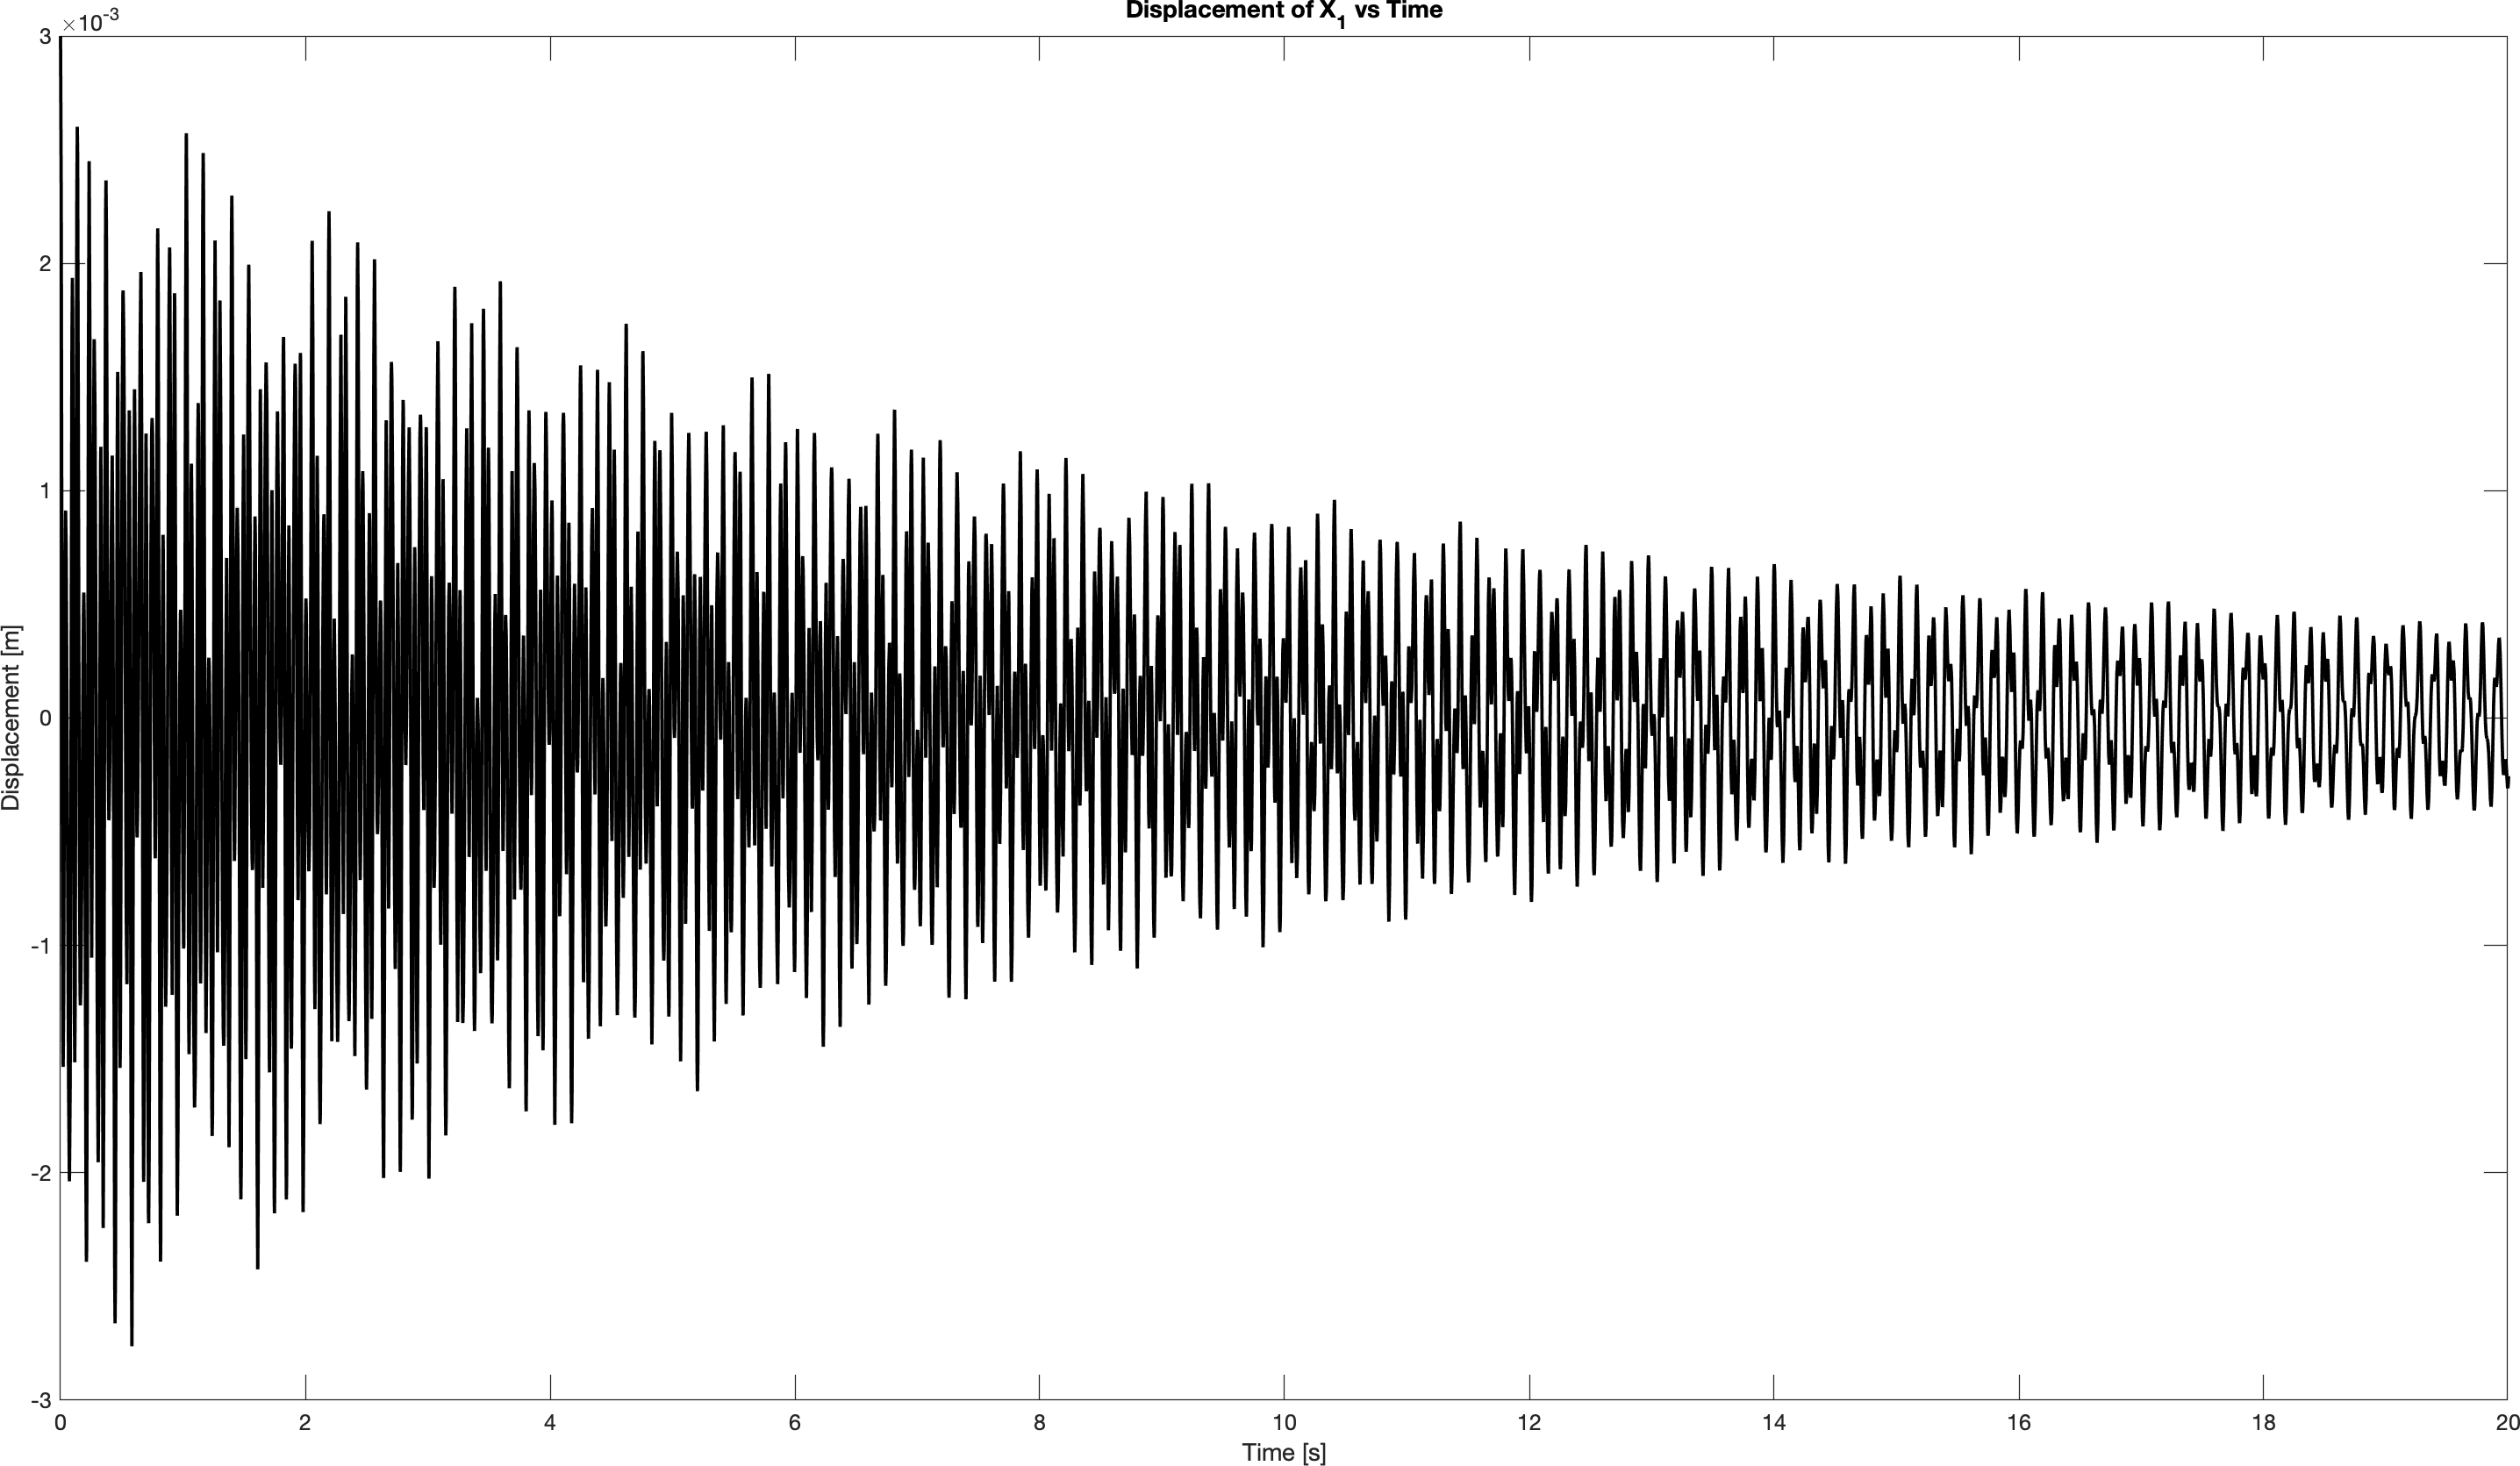
\includegraphics[width=1\textwidth,left]{MCHE 6390/Project 1/Figures/Figure_1.png}
    \captionsetup{justification=raggedright,singlelinecheck=false}
    \caption{Displacement of $x_1$ over time}
    \label{fig:x_1}
\end{figure}

\begin{figure}[H]
    \vspace{-10pt}
    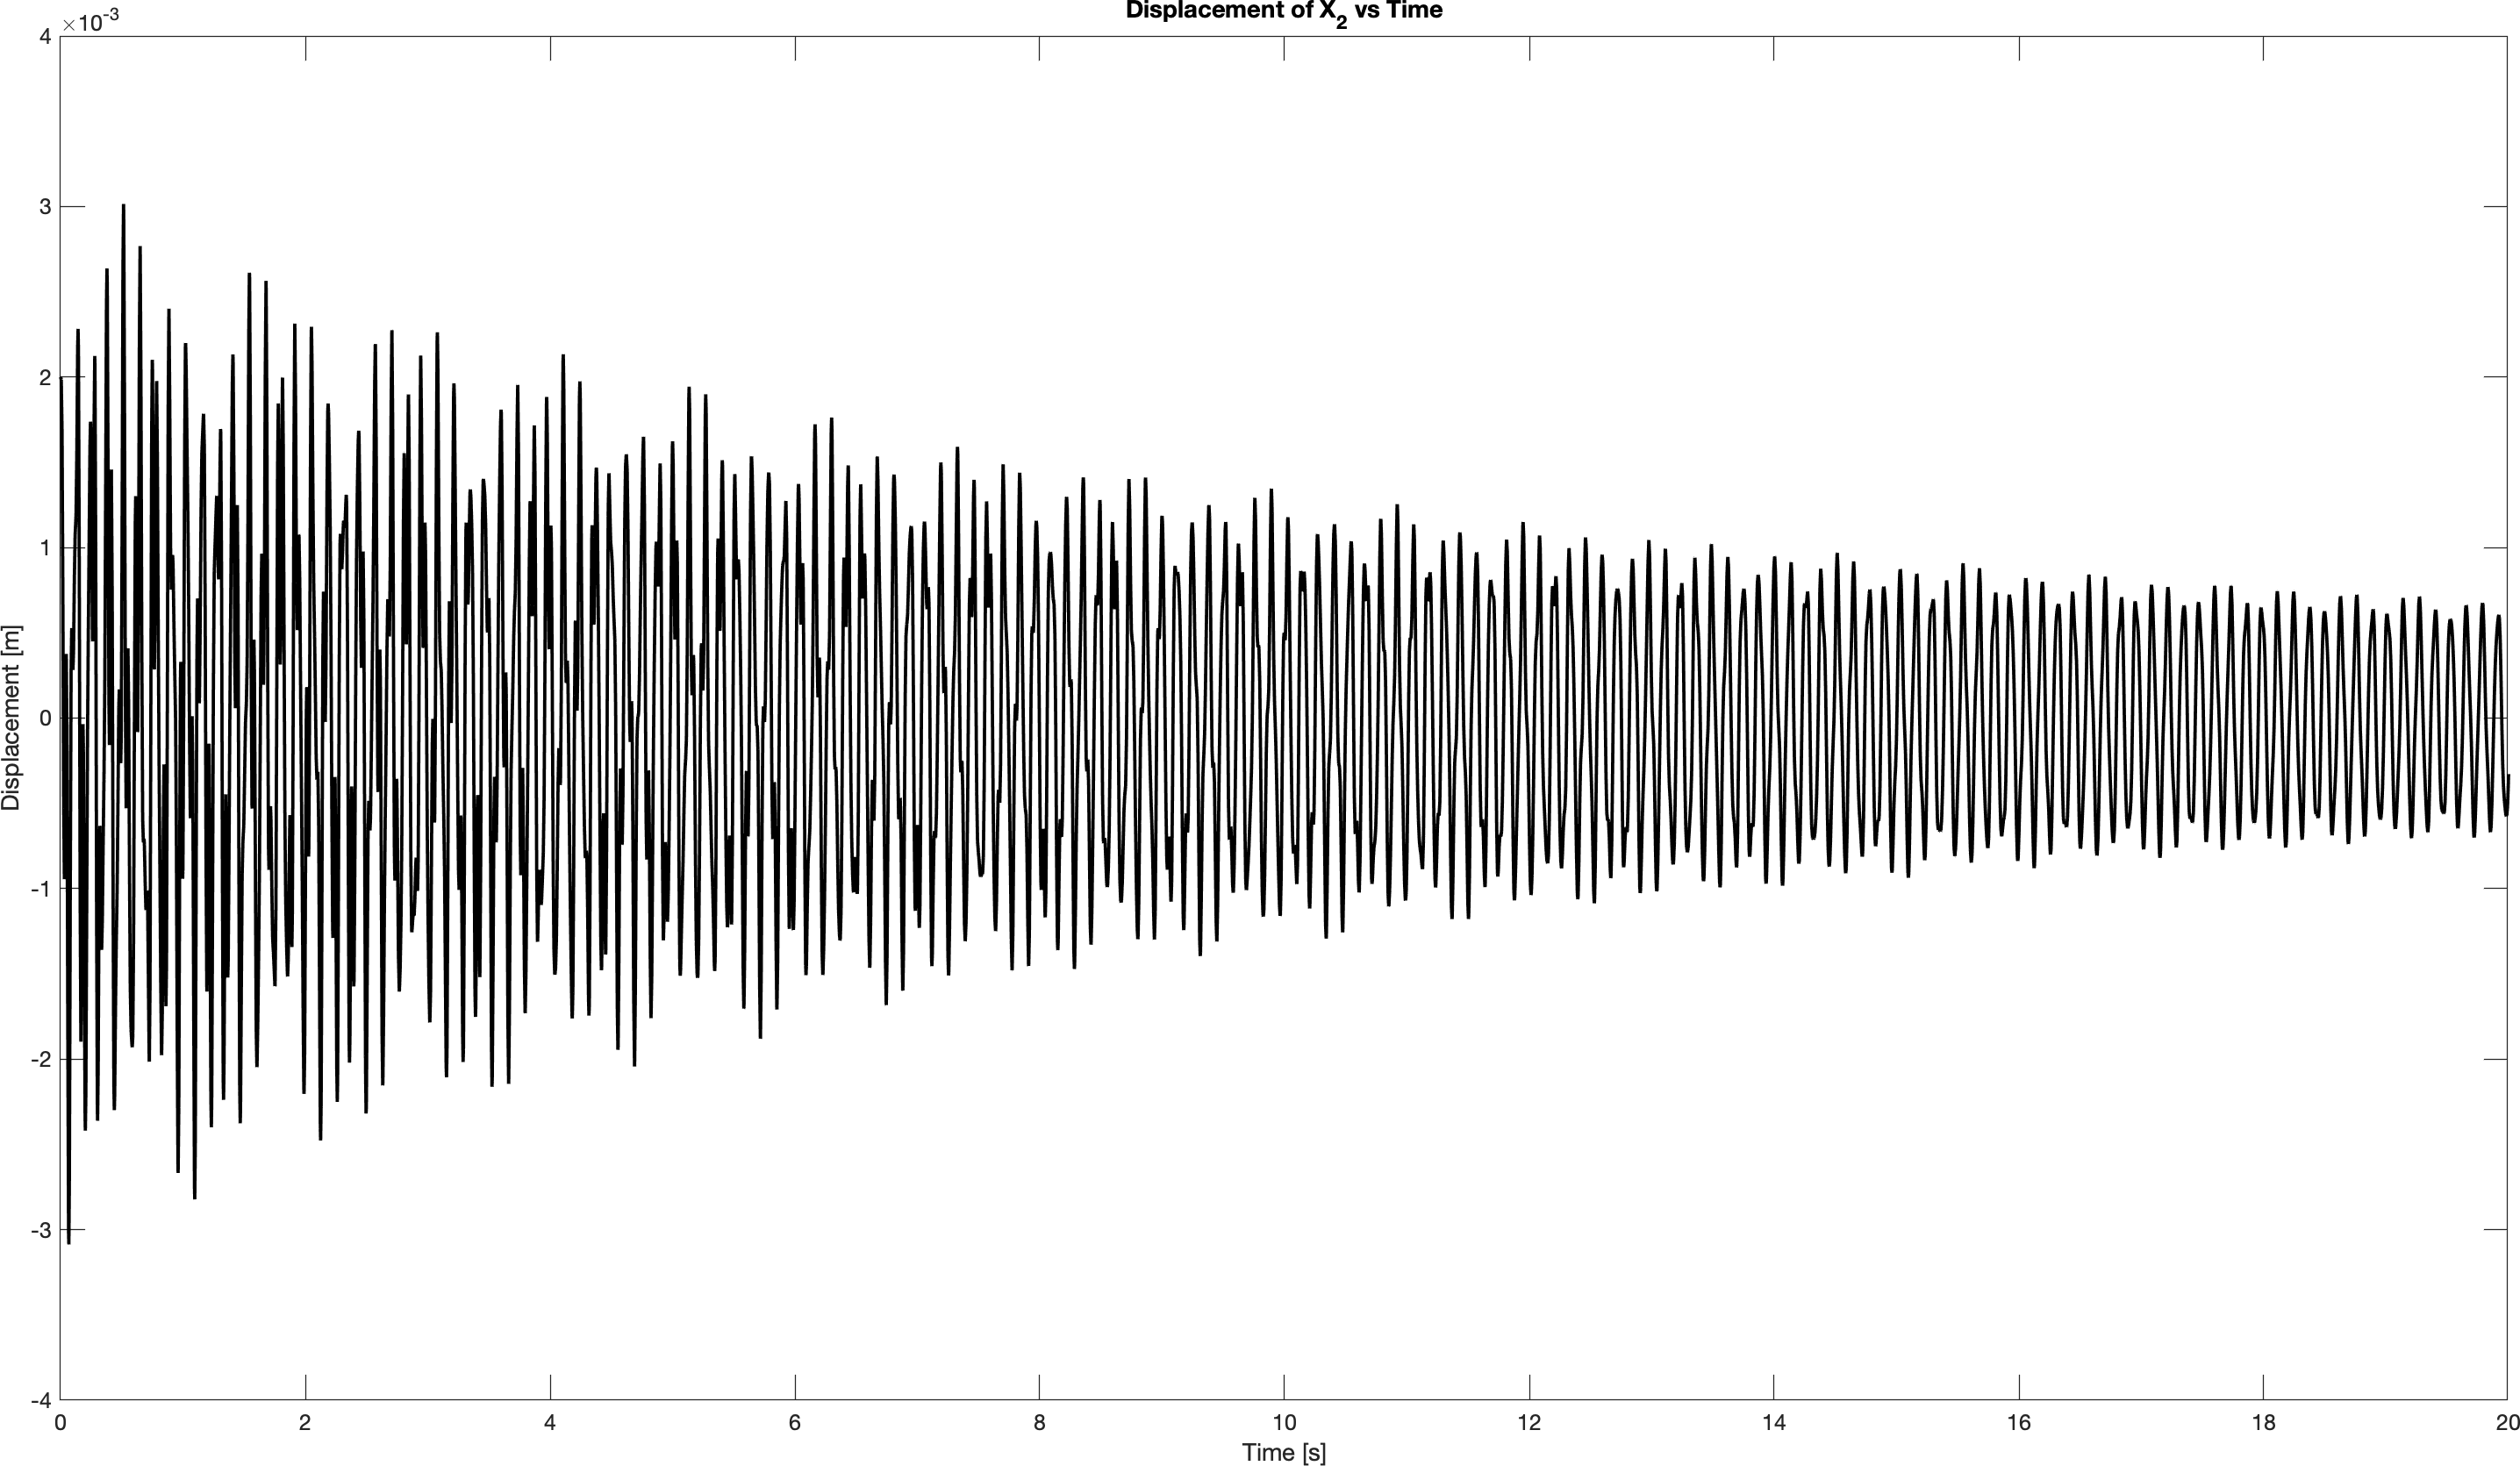
\includegraphics[width=1\textwidth,left]{MCHE 6390/Project 1/Figures/Figure_2.png}
    \captionsetup{justification=raggedright,singlelinecheck=false}
    \caption{Displacement of $x_2$ over time}
    \label{fig:x_2}
\end{figure}

\begin{figure}[H]
    \vspace{-10pt}
    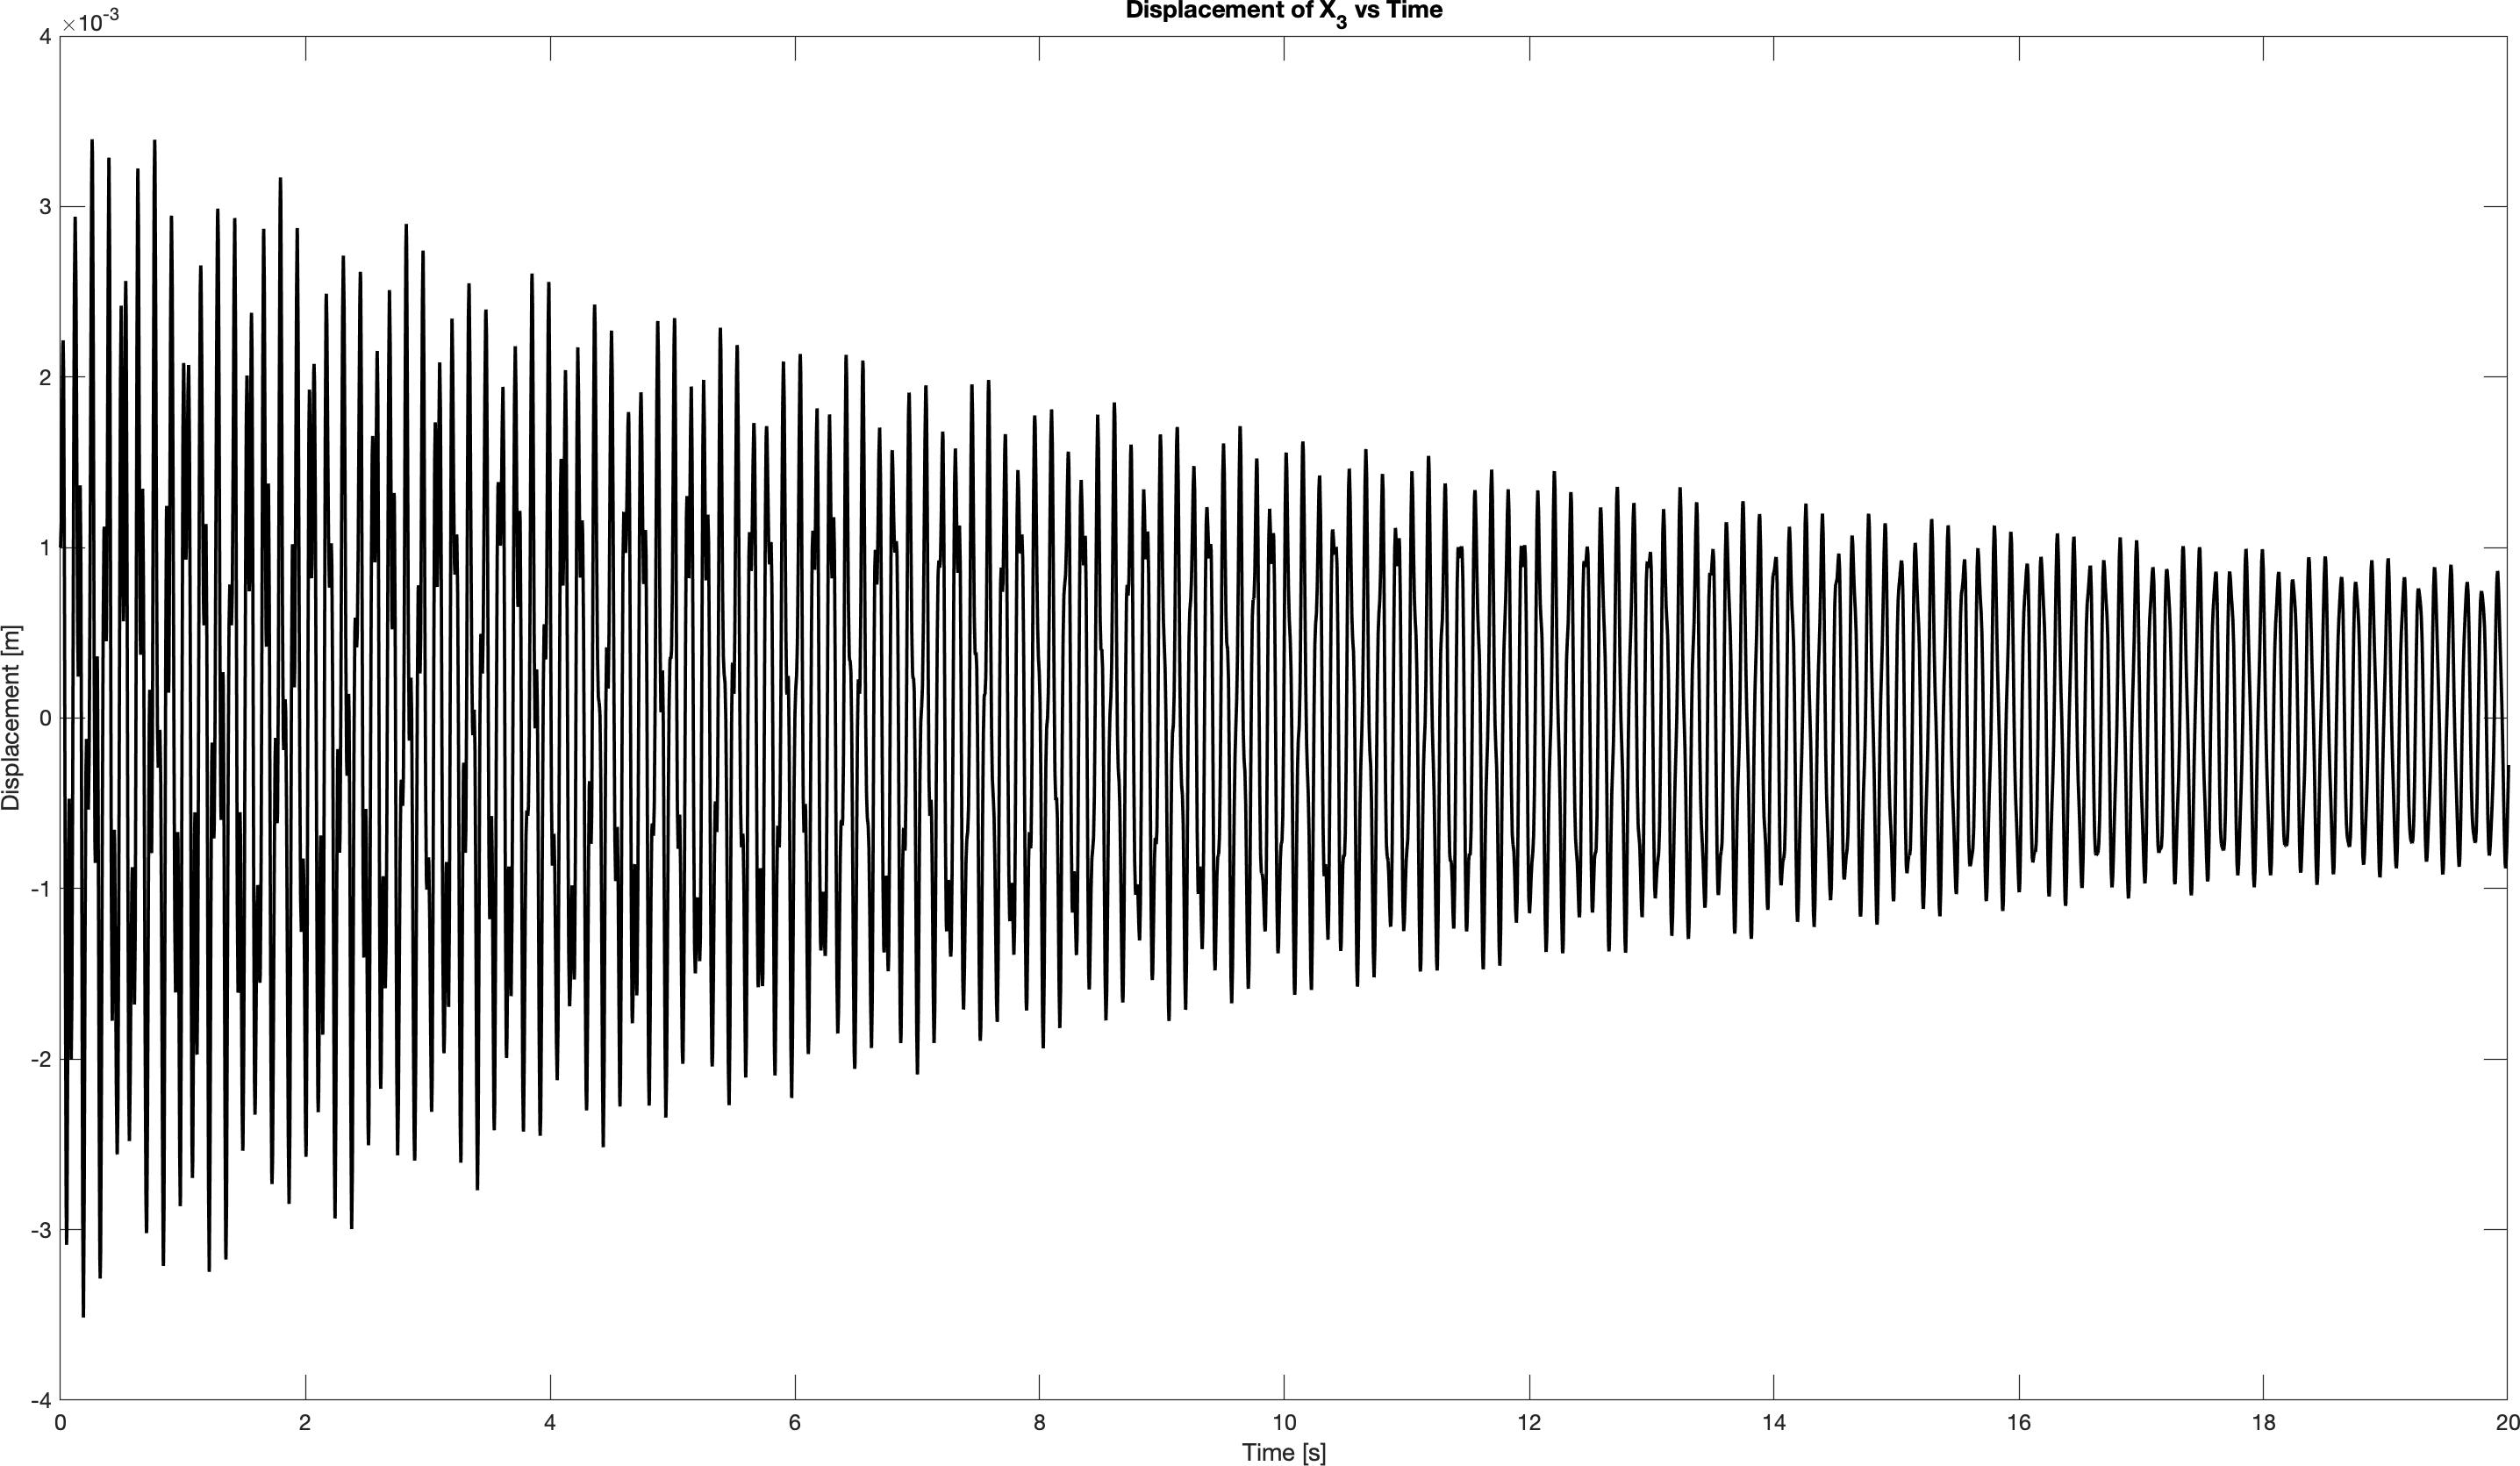
\includegraphics[width=1\textwidth,left]{MCHE 6390/Project 1/Figures/Figure_3.png}
    \captionsetup{justification=raggedright,singlelinecheck=false}
    \caption{Displacement of $x_3$ over time}
    \label{fig:x_3}
\end{figure}

\subsection*{Part 2}

We now analyze a system with the following initial conditions:
\begin{flalign*}
    \begin{bmatrix}
    x_{1} \\
    x_{2} \\
    x_{3}     
    \end{bmatrix}
    &=
    \begin{bmatrix}
      0 \\
      0 \\
      0
    \end{bmatrix}\times 10^{-3}\text{m}&& \\
    \begin{bmatrix}
    \dot{x}_{1} \\
    \dot{x}_{2} \\
    \dot{x}_{3}     
    \end{bmatrix}
    &=
    \begin{bmatrix}
      0 \\
      0 \\
      0
    \end{bmatrix}\times 10^{-3}\text{m/s}.
\end{flalign*}

In addition to these initial conditions, we will apply a force to the third floor with the form
\begin{flalign*}
    F(t) =
    \begin{cases}
    0   \text{ N} & \text{if $t<0$} \\ 
    100 \text{ N} & \text{if $t=0$} \\
    0   \text{ N} & \text{if $t>0$} \\
    \end{cases}.
\end{flalign*}

\begin{figure}[H]
    \vspace{-10pt}
    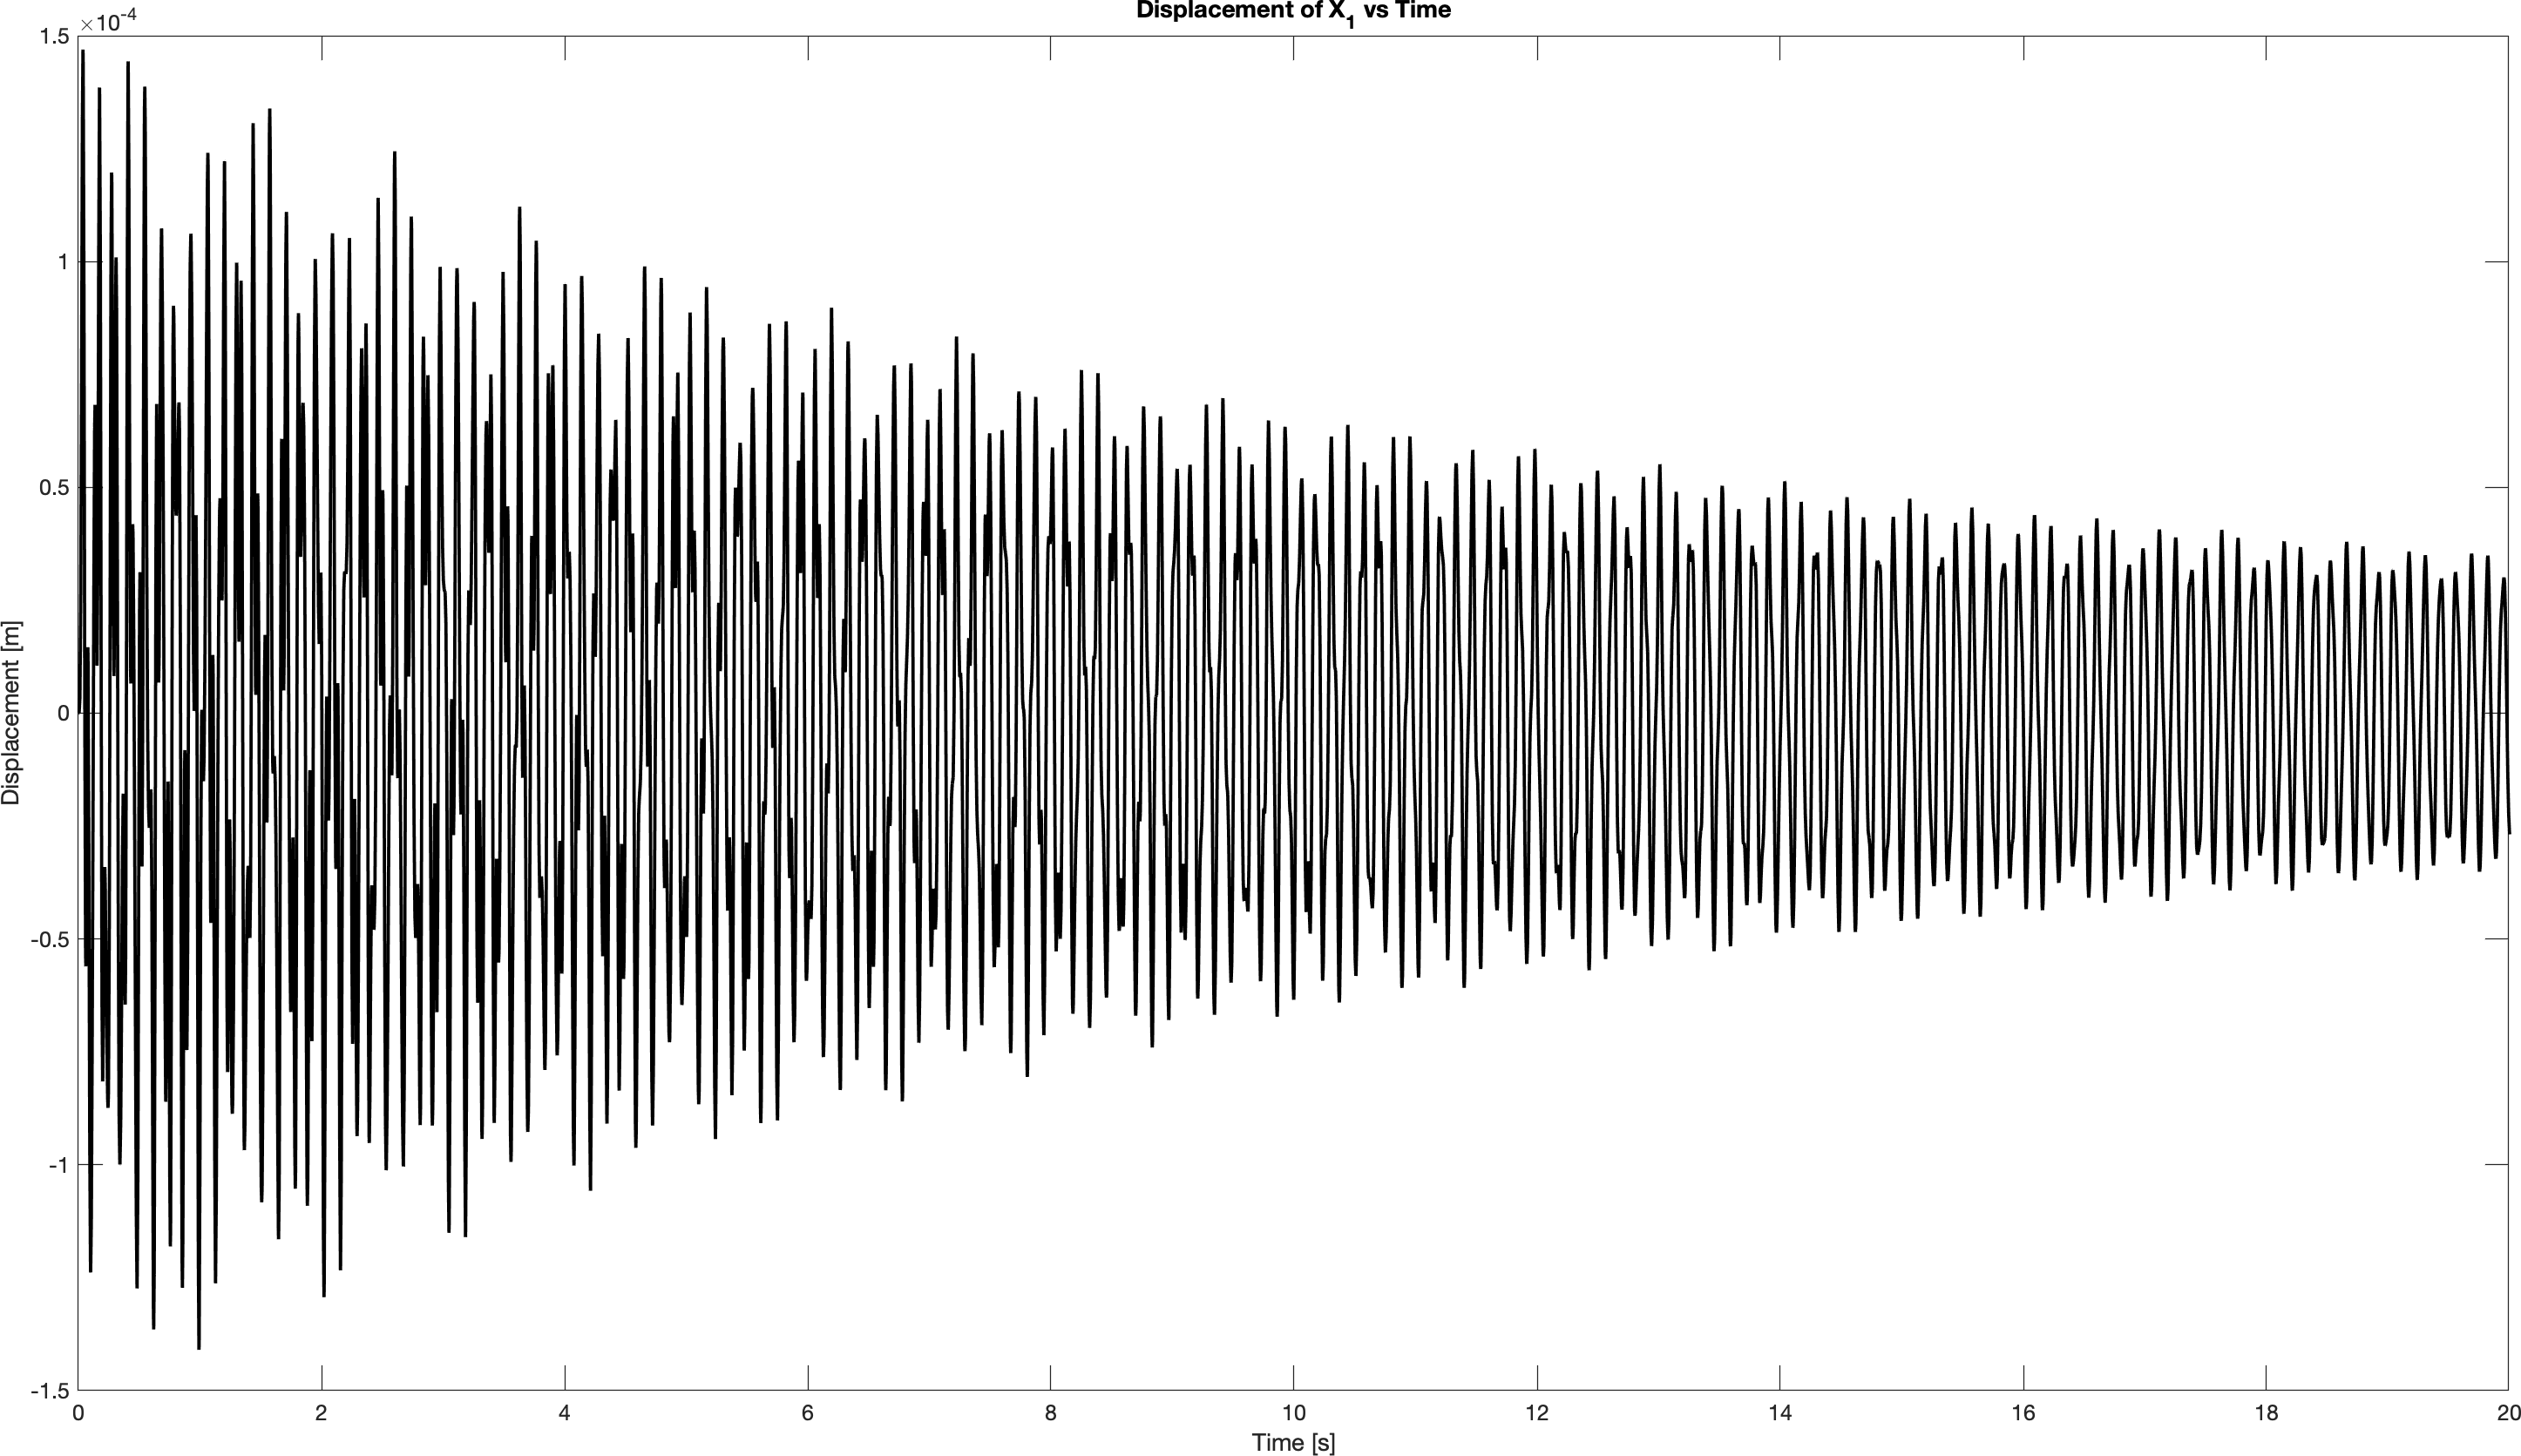
\includegraphics[width=1\textwidth,left]{MCHE 6390/Project 1/Figures/Figure_4.png}
    \captionsetup{justification=raggedright,singlelinecheck=false}
    \caption{Displacement of $x_1$ over time}
    \label{fig:x_1_forced}
\end{figure}

\begin{figure}[H]
    \vspace{-10pt}
    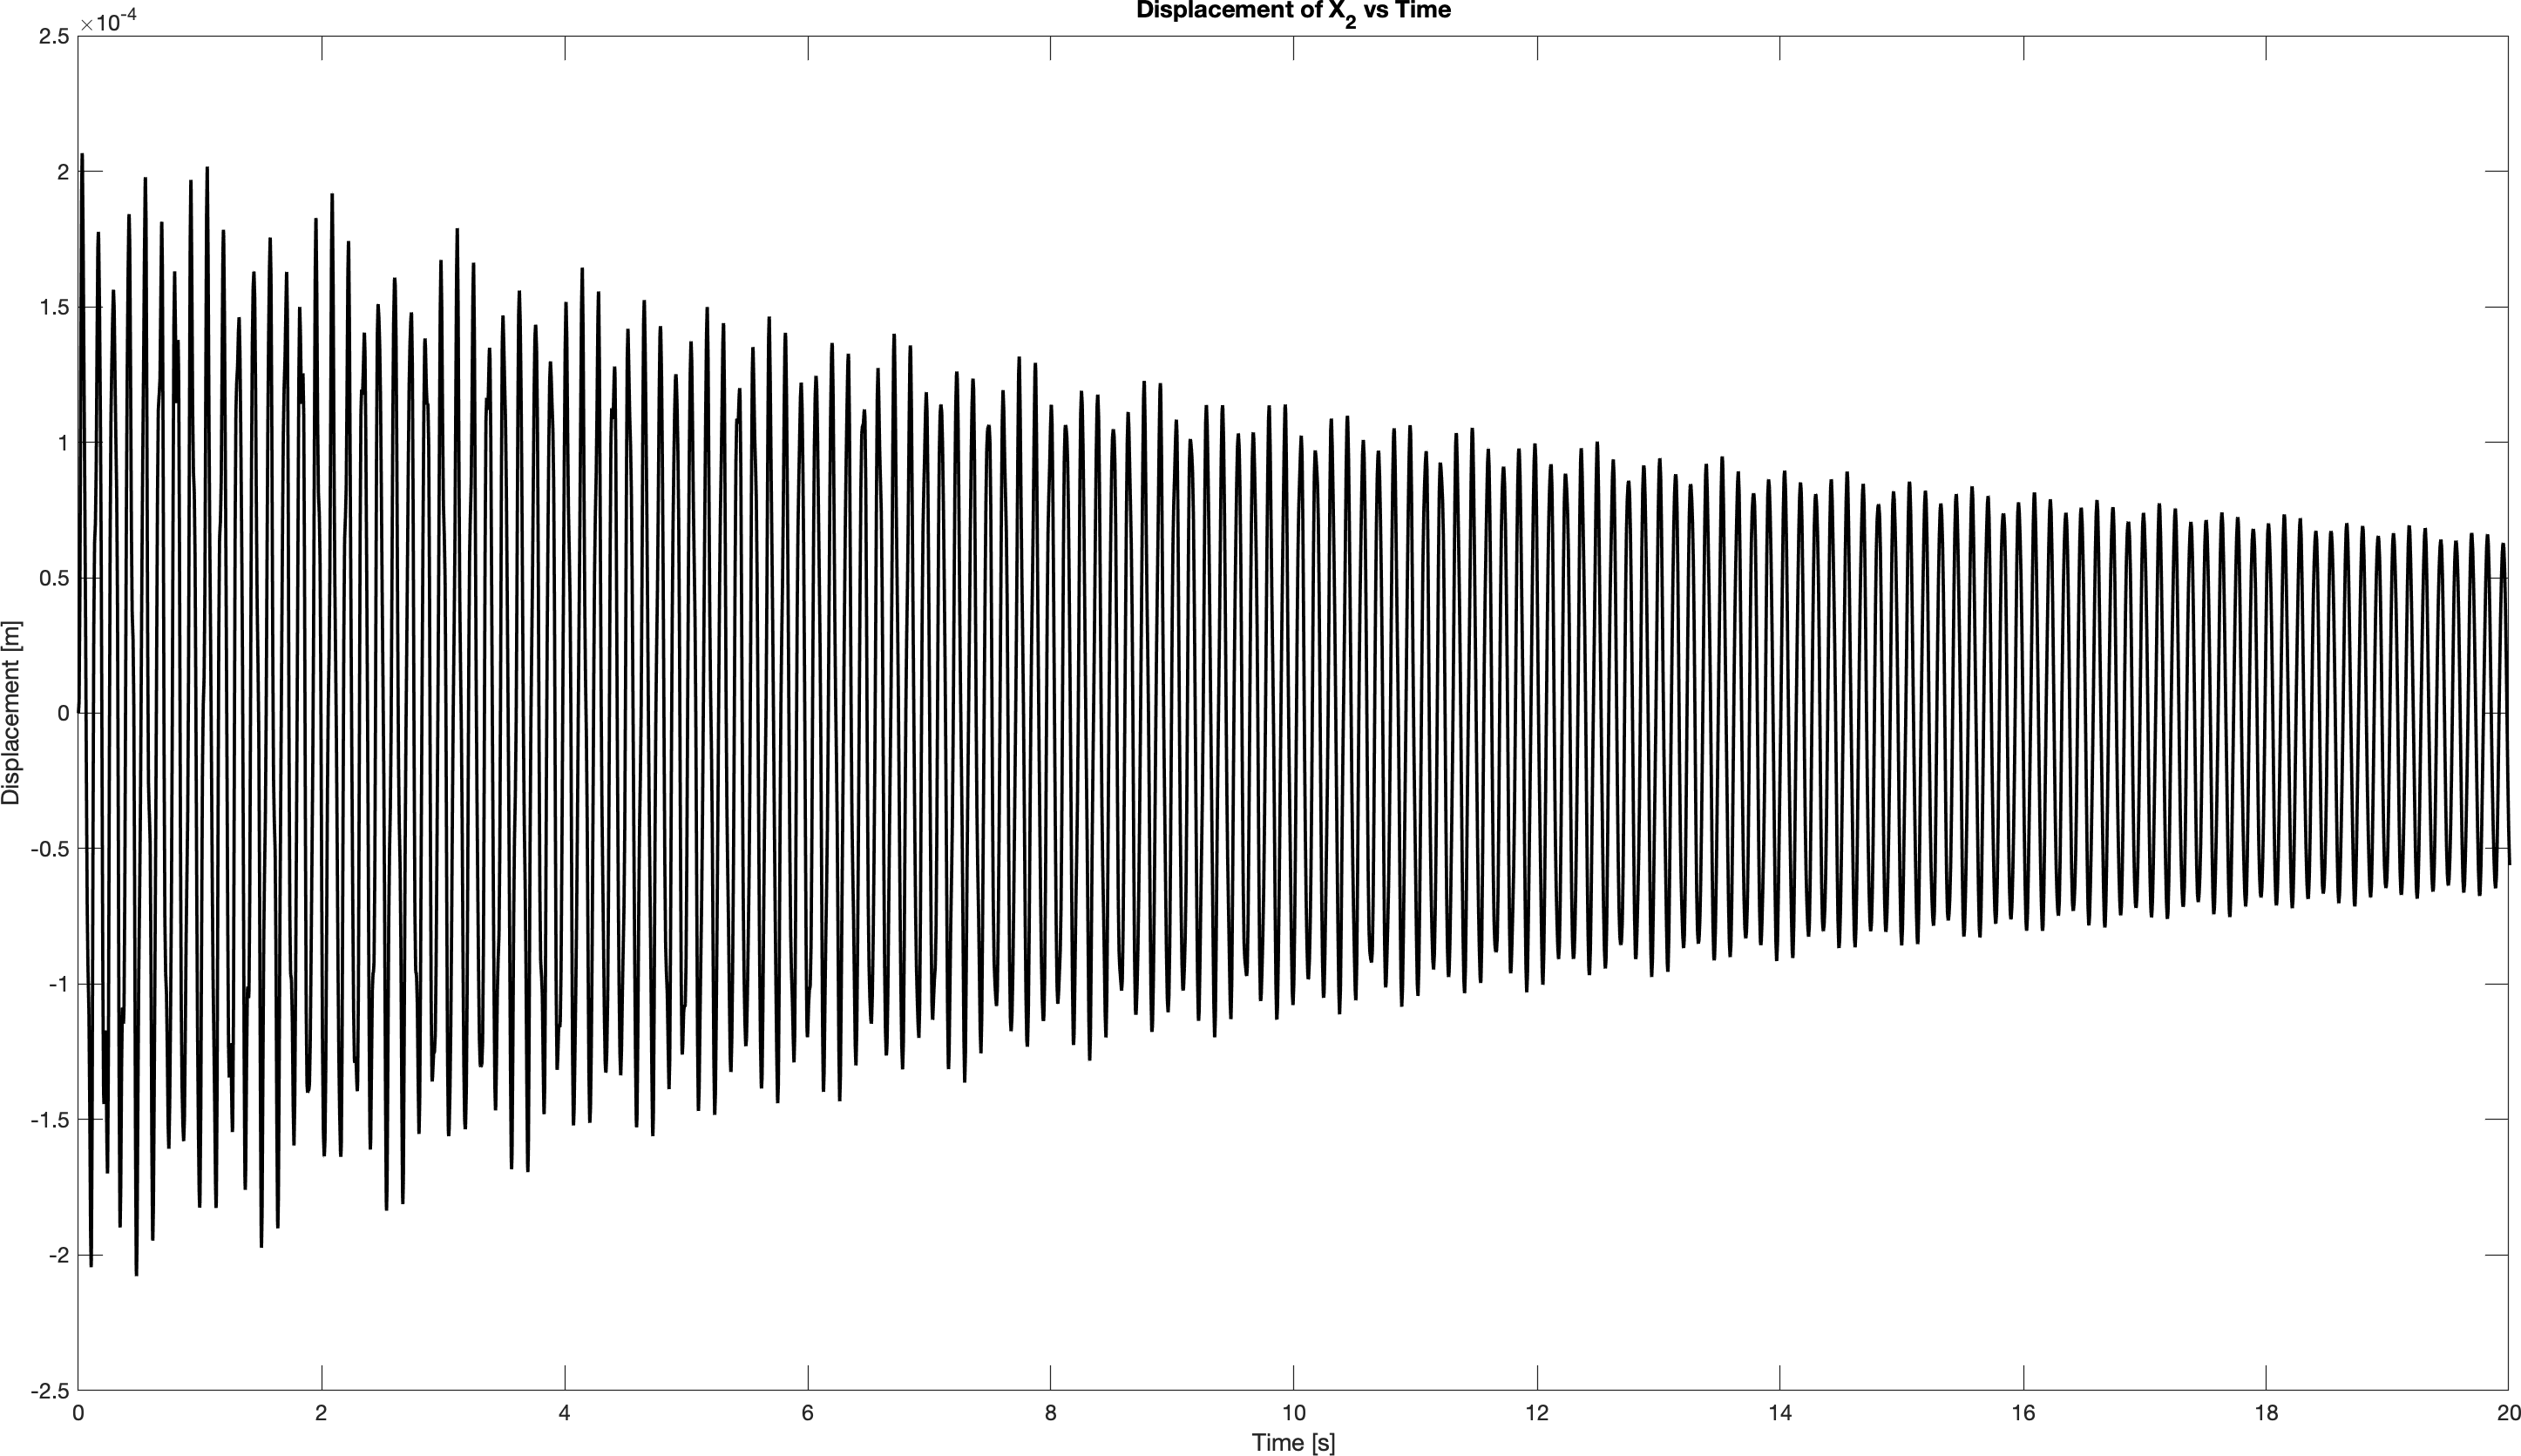
\includegraphics[width=1\textwidth,left]{MCHE 6390/Project 1/Figures/Figure_5.png}
    \captionsetup{justification=raggedright,singlelinecheck=false}
    \caption{Displacement of $x_2$ over time}
    \label{fig:x_2_forced}
\end{figure}

\begin{figure}[H]
    \vspace{-10pt}
    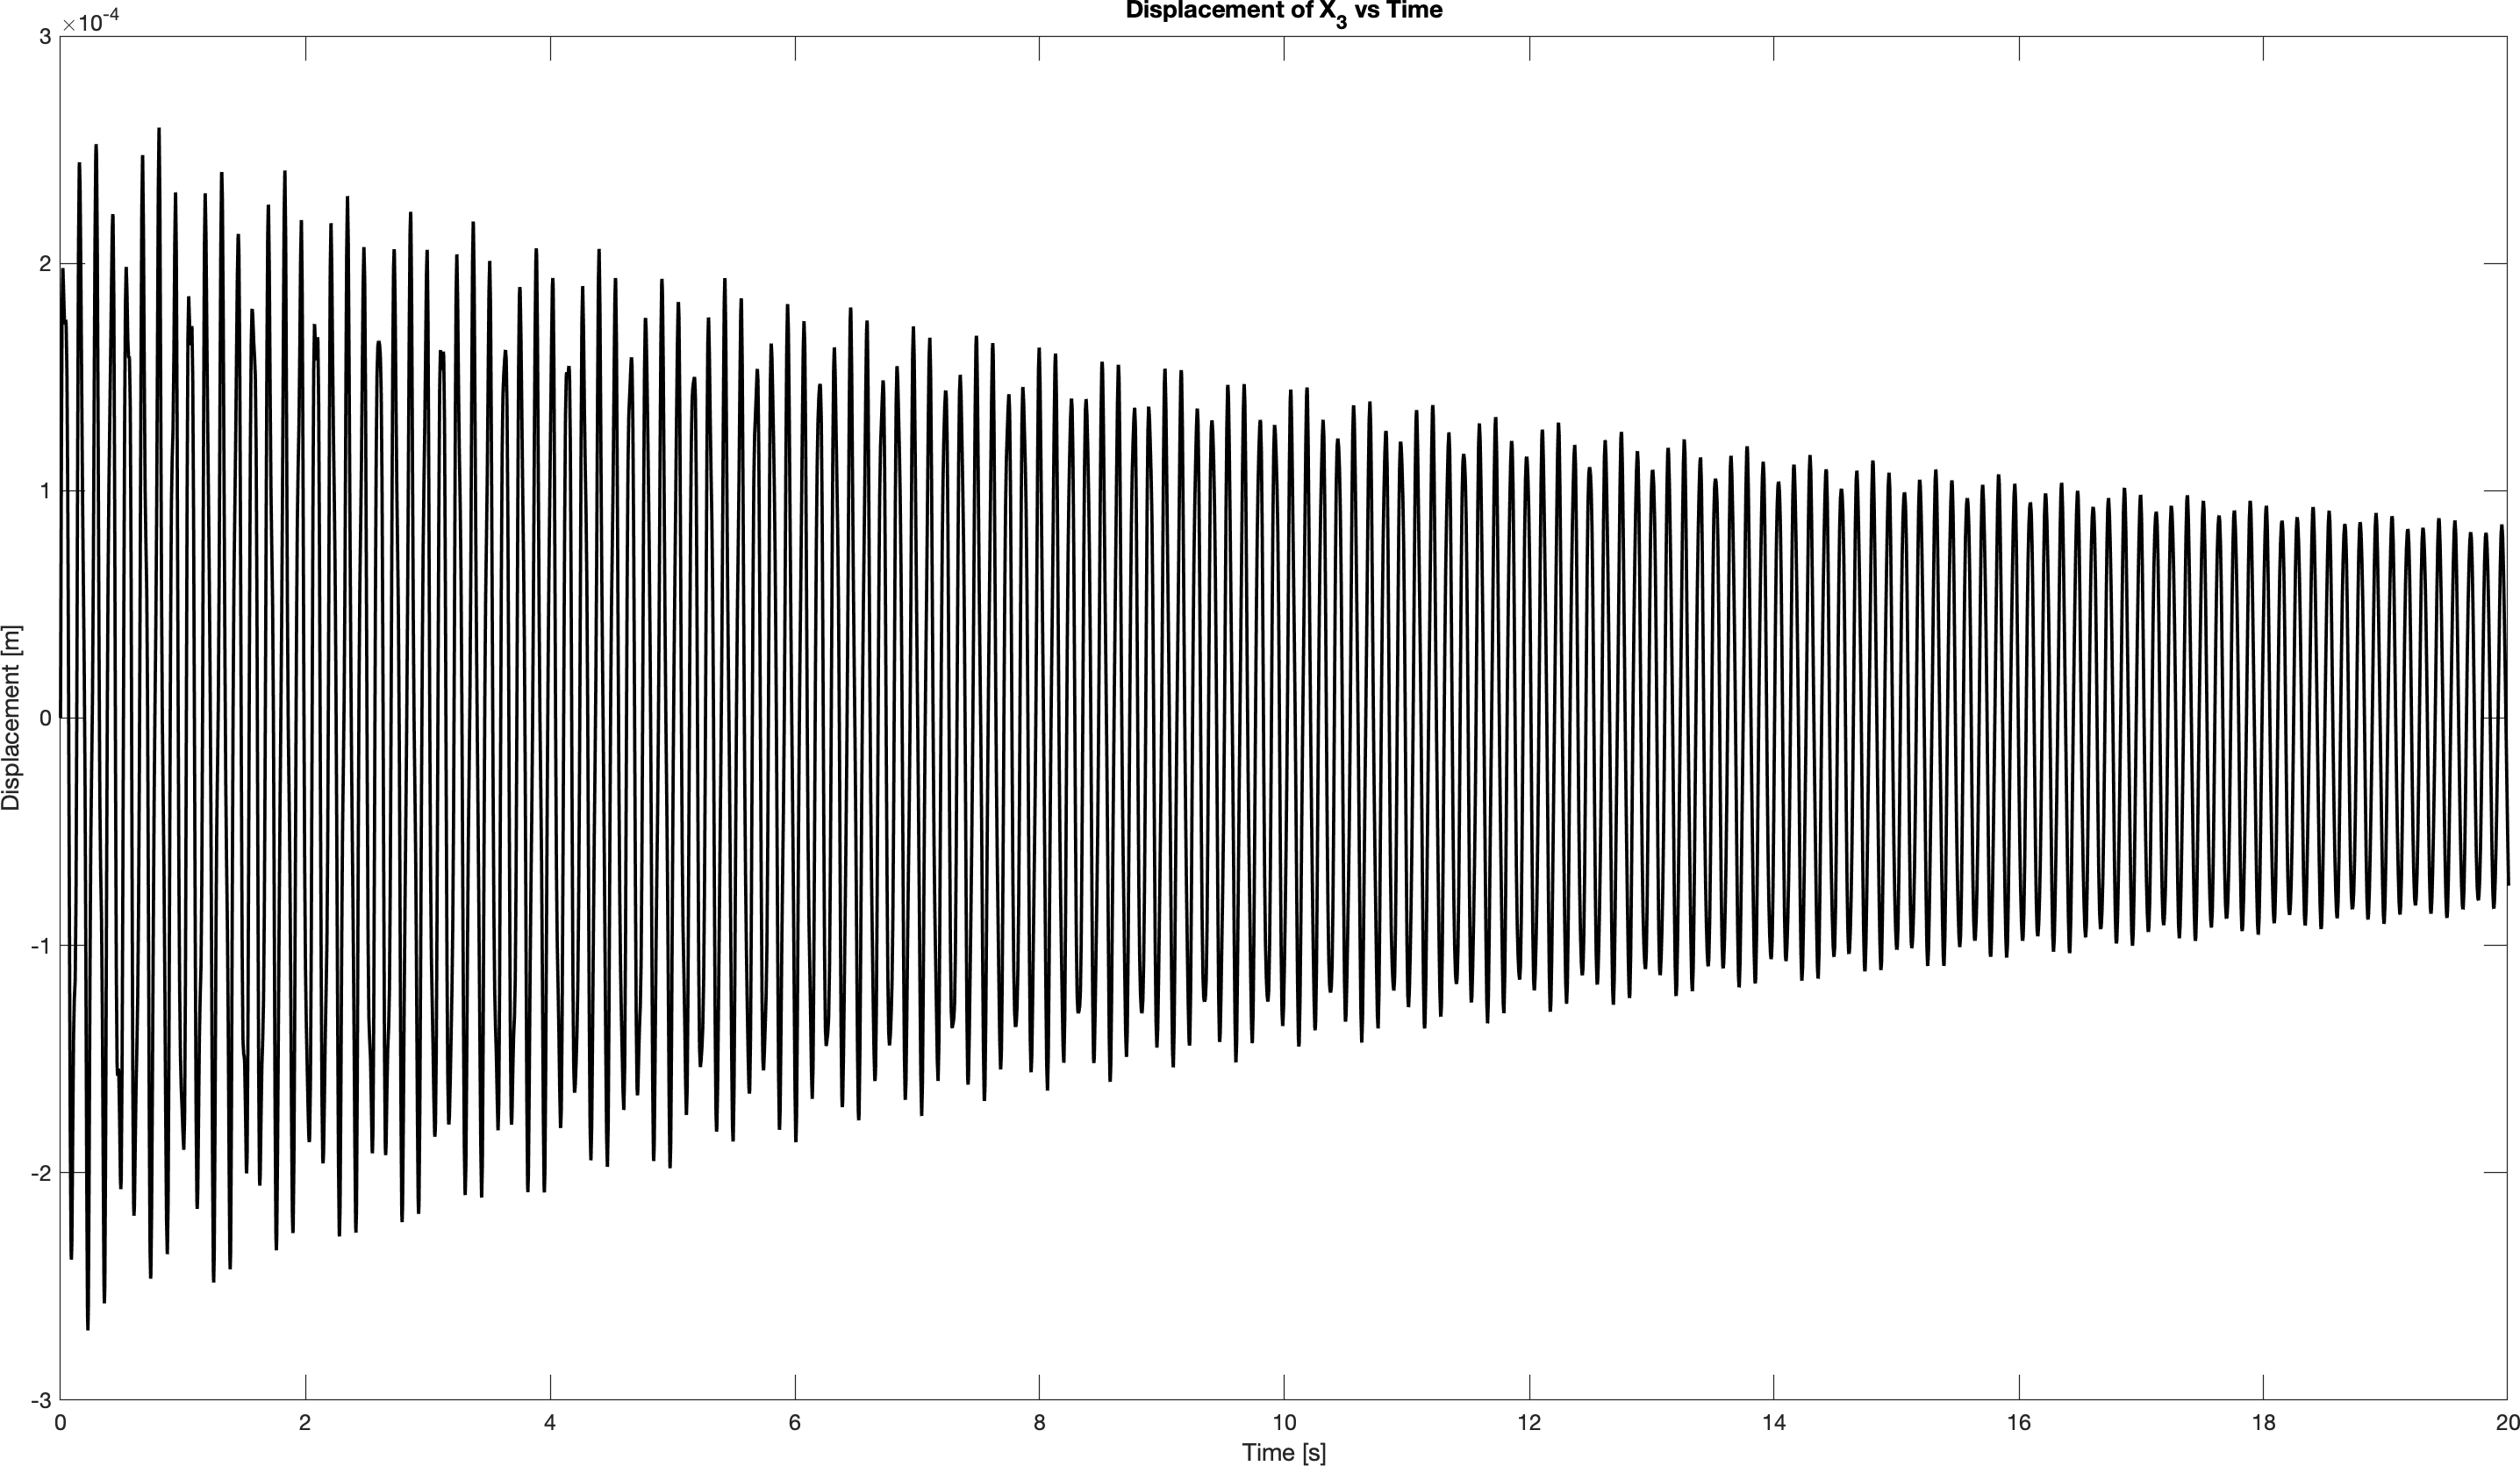
\includegraphics[width=1\textwidth,left]{MCHE 6390/Project 1/Figures/Figure_6.png}
    \captionsetup{justification=raggedright,singlelinecheck=false}
    \caption{Displacement of $x_3$ over time}
    \label{fig:x_3_forced}
\end{figure}

\section*{Appendix}
\subsection*{MCHE\_6390\_MDOF.m}
\begin{lstlisting}[style=Matlab-editor]
function [X,L,U] = MCHE_6390_MDOF(M,K,Z,F,B_f,IC_p,IC_v,t,Options)
%   MCHE_6390

% Ensure number of arguments is correct
narginchk(8,9);
nargoutchk(0,3);

% Convert string to character arrays
if nargin > 8
    Options = convertStringsToChars(Options);
else
    Options = 'NoOptions';
end

[Mn,~] = size(M);

% Validate attributes of inputs
validateattributes(F,{'function_handle'},{'real'});
validateattributes(M,{'single','double'},{'real','finite','square',...
    'nonnegative'});
validateattributes(K,{'single','double'},{'real','finite','square',...
    'size',[Mn,Mn]});
validateattributes(Z,{'single','double'},{'real','finite','size',...
    [Mn,1],'>=',0,'<=',1});
validateattributes(IC_p,{'single','double'},{'real','finite','size',...
    [Mn,1]});
validateattributes(IC_v,{'single','double'},{'real','finite','size',...
    [Mn,1]});
validateattributes(t,{'single','double'},{'real','finite','size',[1,NaN]});

test = F(t(end));
[testp,~] = size(test);

validateattributes(B_f,{'single','double'},{'binary','size',...
    [Mn,testp]});

% Solve generalized eigenvalue problem
[U_I,L_I] = eig(K,M);

% Select diagonal entries from L_I.^0.5 and sort them in increasing order
[L,I] = sort(diag(L_I.^0.5));

% Initialize U
U = zeros(length(M),length(M));

% Mass normalize U
for i = 1:length(M)
    U(:,i) = U_I(:,I(i))./sqrt((U_I(:,i)'*M*U_I(:,i)));
end

% Calculate Psi
Psi = U'*B_f;

% Calculate Modal Initial Conditions
r_0 = (U^-1)*IC_p;
r_0_dot = (U^-1)*IC_v;

% Calculate A and phi
A = sqrt((((r_0_dot+Z.*L.*r_0).^2)+((r_0.*L.*sqrt(1-Z.^2)).^2))./...
    ((L.*sqrt(1-Z.^2)).^2));
phi = atan2(L.*sqrt(1-Z.^2).*r_0,r_0_dot+Z.*L.*r_0);

% Initialize X_H
X_H = zeros(length(t),length(M));

for i = 1:length(t)
    X_H(i,:) = U*(A.*exp(-Z.*L*t(i)).*sin(L.*sqrt(1-Z.^2)*t(i)+phi));
end

X_P = zeros(length(t),length(M));

for i = 1:length(t)
    X_P(i,:) = U*Convolution(F,L,L.*sqrt(1-Z.^2),Z,t(i),Psi);
end

X = X_P'+X_H';

if isequal(Options,'Plot')
    figure(1)
    plot(t,X_H(1,:))
    
    figure(2)
    plot(t,X_P(1,:))
    
    figure(3)
    plot(t,X(1,:))
end

function C = Convolution(f,wn,wd,z,t,Psi)

% Impulse response
g = @(t,tau,wn,wd,z) (1./wd).*exp(-z.*wn*(t-tau)).*sin(wd*(t-tau));

% Compute convolution, sum over p
C = sum(Psi.*(integral(@(tau) g(t,tau,wn,wd,z)*f(tau)',0,t,...
    'ArrayValued',true)),2);
\end{lstlisting}
\newpage
\subsection*{MCHE\_6390\_Project\_1\_Prelab.m}
\begin{lstlisting}[style=Matlab-editor]
% Given values
b = 3.81*(10^-2);
h = 3.175*(10^-3);
rho = 8050;
E = 200*10^9;
l = [27.15*10^-2;29.53*10^-2;29.53*10^-2];
L1 = 30.48*10^-2;
L2 = 15.24*10^-2;
L3 = 9.525*10^-3;

% K
K_eq = 4*E*b*((h./l).^3);
K = [K_eq(1)+K_eq(2), -K_eq(2),0;-K_eq(2), K_eq(2)+K_eq(3),-K_eq(3);0,...
    -K_eq(3),K_eq(3)];
      
% M
M = L1*L2*L3*rho*eye(3);

% Z
Z = 0.001*ones(3,1);

%% Free Response
F = @(t) 0*t;
B_f = zeros(3,1);
IC_p = [3;2;1]*10^-3;
IC_v = zeros(3,1);
Options = '';
t = linspace(0,20,30000);

[X,L,U] = MCHE_6390_MDOF(M,K,Z,F,B_f,IC_p,IC_v,t,Options);

disp(L)
disp(U)

figure(1)
% Plot
plot(t,X(1,:),'-k','LineWidth',1.5);
% limits
xlim([0 t(end)])
% Title and axis labels
title('Displacement of X_1 vs Time')
xlabel('Time [s]')
ylabel('Displacement [m]')
% Make plot size of computer screen
set(gcf, 'Units', 'Normalized', 'OuterPosition', [0 0 1 1]);
% Set background color to white
set(gcf, 'Color', 'w');
export_fig Figure_1.png -m2.5

figure(2)
% Plot
plot(t,X(2,:),'-k','LineWidth',1.5);
% limits
xlim([0 t(end)])
% Title and axis labels
title('Displacement of X_2 vs Time')
xlabel('Time [s]')
ylabel('Displacement [m]')
% Make plot size of computer screen
set(gcf, 'Units', 'Normalized', 'OuterPosition', [0 0 1 1]);
% Set background color to white
set(gcf, 'Color', 'w');
export_fig Figure_2.png -m2.5

figure(3)
% Plot
plot(t,X(3,:),'-k','LineWidth',1.5);
% limits
xlim([0 t(end)])
% Title and axis labels
title('Displacement of X_3 vs Time')
xlabel('Time [s]')
ylabel('Displacement [m]')
% Make plot size of computer screen
set(gcf, 'Units', 'Normalized', 'OuterPosition', [0 0 1 1]);
% Set background color to white
set(gcf, 'Color', 'w');
export_fig Figure_3.png -m2.5

%% Forced Response

F = @(T) Impulse(T,t(2),100);
B_f = [0;0;1];
IC_p = zeros(3,1);
IC_v = zeros(3,1);
Options = '';

[X,L,U] = MCHE_6390_MDOF(M,K,Z,F,B_f,IC_p,IC_v,t,Options);

figure(4)
% Plot
plot(t,X(1,:),'-k','LineWidth',1.5);
% limits
xlim([0 t(end)])
% Title and axis labels
title('Displacement of X_1 vs Time')
xlabel('Time [s]')
ylabel('Displacement [m]')
% Make plot size of computer screen
set(gcf, 'Units', 'Normalized', 'OuterPosition', [0 0 1 1]);
% Set background color to white
set(gcf, 'Color', 'w');
export_fig Figure_4.png -m2.5

figure(5)
% Plot
plot(t,X(2,:),'-k','LineWidth',1.5);
% limits
xlim([0 t(end)])
% Title and axis labels
title('Displacement of X_2 vs Time')
xlabel('Time [s]')
ylabel('Displacement [m]')
% Make plot size of computer screen
set(gcf, 'Units', 'Normalized', 'OuterPosition', [0 0 1 1]);
% Set background color to white
set(gcf, 'Color', 'w');
export_fig Figure_5.png -m2.5   

figure(6)
% Plot
plot(t,X(3,:),'-k','LineWidth',1.5);
% limits
xlim([0 t(end)])
% Title and axis labels
title('Displacement of X_3 vs Time')
xlabel('Time [s]')
ylabel('Displacement [m]')
% Make plot size of computer screen
set(gcf, 'Units', 'Normalized', 'OuterPosition', [0 0 1 1]);
% Set background color to white
set(gcf, 'Color', 'w');
export_fig Figure_6.png -m2.5

function [F] = Impulse(T,T_end,Mag)

F = zeros(length(T),1);

for i = 1:length(T)
    if T(i)<T_end
        F(i) = max(Mag);
    else
        F(i) = 0;
    end
end

end
\end{lstlisting}
\end{document}
